\subsection{群芽的情形}

设 \((\mathbf{G}, e, \theta, m)\) 为李群芽，\(\Omega\) 为 m 的定义集。于是 \(\mathrm{T}(\Omega)\) 与 \(\mathrm{T}(\mathrm{G}) \times \mathrm{T}(\mathrm{G})\) 的一个开子集认同，而 \(\mathrm{T}(m)\) 是从 T(Ω) 到 T(G) 的解析映射。可以像第 2 节那样验证 (T(G), 0e, T(θ), T(m)) 是李群芽。G 与 T(G) 的乘法通常用乘法记号书写。T(G) 到 G 上的典范投影是李群芽态射。Te(m) 在 Te(G) 上的限制是 Te(G) 的向量空间加法。T(G) 的零截面是李群芽 G 到 T(G) 的一个李子群芽上的同构，我们把该李子群芽与 G 认同。若 f 是 G 到李群芽 H 的态射，则 T(f): T(G) → T(H) 是李群芽态射。

映射 \(\phi\colon(g,u)\mapsto gu\)（从 \(G\times T_{e}(G)\) 到 \(T(G)\)）是平凡向量丛 \(G\times T_{e}(G)\)（底空间为 \(G\)）到向量丛 \(T(G)\) 上的同构；因为 \(\phi\) 与 \(\phi^{-1}\) 都是解析的且都是向量丛态射，故只需引用 Differentiable and Analytic Manifolds, R, 7.2.1。（第 2 节的证明经过改动也可移用于此。）同构 \(\phi^{-1}\) 称为 \(T(G)\) 的左平凡化。映射 \((g,u)\mapsto ug\) 的逆同构称为右平凡化。

设 X 为 \(C^{r}\) 类流形，\(\psi\) 为 G 在 X 上的一个 \(C^{r}\) 类左作用律片段。于是 \(\mathrm{T}(\psi)\) 是一个 \(C^{r-1}\) 类的、\(\mathrm{T}(\mathrm{G})\) 在 T(X) 上的左作用律片段，且它是 \(\psi\) 的扩充。只要 gx 有定义，公式 (7)、(8) 与 (9) 便仍然有效。若 I 是 K 中包含 0 的开子集，若 \(\gamma: I \to G\) 是 \(C^{r}\) 类映射且满足 \(\gamma(0) = e\)，且若 \(a = \mathrm{T}_{0}(\gamma)1\)，则在 X 上定义的向量场 \(x \mapsto ax\) 就是 Differentiable and Analytic Manifolds, R, 8.4.5 意义下由映射 \((\lambda, x) \mapsto \gamma(\lambda)x\) 所定义的向量场。

\section{从李群过渡到它的李代数}

\subsection{李群上点分布的卷积}

定义 1. 设 G 为李群，g 与 \(g'\) 为 G 的两点，且设 \(t \in \mathrm{T}_{g}^{(\infty)}(\mathrm{G})\)、\(t' \in \mathrm{T}_{g'}^{(\infty)}(\mathrm{G})\) 为 G 上在 g 与 \(g'\) 处的两个点分布 (Differentiable and Analytic Manifolds, R, 13.2.1)。t 与 \(t'\) 的卷积，记作 \(t * t'\)，是 \(t \otimes t'\) 在 G × G 到 G 的映射 \((h, h') \mapsto hh'\) 下的像 (Differentiable and Analytic Manifolds, R, 13.2.3)。

命题 1. (i) 若 \(t \in \mathrm{T}_g^{(s)}(\mathrm{G})\) 且 \(t' \in \mathrm{T}_{g'}^{(s')}(\mathrm{G})\)，则 \(t * t' \in \mathrm{T}_{gg'}^{(s + s')}(\mathrm{G})\)。

\begin{enumerate}
\def\labelenumi{(\roman{enumi})}
\setcounter{enumi}{1}
\tightlist
\item
  若 \(t\) 或 \(t'\) 没有常数项，则 \(t * t'\) 没有常数项。
\end{enumerate}

\[
\varepsilon_ {g} * \varepsilon_ {g ^ {\prime}} = \varepsilon_ {g g ^ {\prime}}.
\]

\begin{enumerate}
\def\labelenumi{(\roman{enumi})}
\setcounter{enumi}{3}
\tightlist
\item
  设 \(t \in \mathrm{T}_g^{(s)}(\mathrm{G})\)，\(t' \in \mathrm{T}_{g'}^{(s')}(\mathrm{G})\)，并设 \(f\) 是取值于一个分离多范空间的 \(\mathbf{C}^{s + s'}\) 类函数，定义在 \(gg'\) 的一个开邻域上。则
\end{enumerate}

\[
\begin{array}{c} \langle t * t ^ {\prime}, f \rangle = \langle t ^ {\prime}, h ^ {\prime} \mapsto \langle t, h \mapsto f (h h ^ {\prime}) \rangle \rangle \\ = \langle t, h \mapsto \langle t ^ {\prime}, h ^ {\prime} \mapsto f (h h ^ {\prime}) \rangle \rangle . \end{array}
\]

这由 Differentiable and Analytic Manifolds, R, 13.4.1、13.2.3 与 13.4.4 得出。

设 K = R 或 C，且 G 是有限维的。于是 G 是局部紧的。若 t、\(t'\) 是点测度，则 \(t \star t'\) 的定义与 Integration, Chapter VIII, § 1 中的定义一致。我们以后将看到，测度的卷积与点分布的卷积是不必为点分布的分布的卷积的两个特殊情形。

设 \(\mathcal{T}^{(\infty)}(\mathrm{G})\) 为诸 \(\mathrm{T}_g^{(\infty)}(\mathrm{G})\)（\(g\in \mathrm{G}\)）的直和 (cf.~Differentiable and Analytic Manifolds, R, 13.6.1)。我们把 \(\mathcal{T}^{(\infty)}(\mathrm{G})\) 的卷积定义为 \(\mathcal{T}^{(\infty)}(\mathrm{G})\times \mathcal{T}^{(\infty)}(\mathrm{G})\) 到 \(\mathcal{T}^{(\infty)}(\mathrm{G})\) 的、是定义 1 的卷积之扩充的双线性映射。我们也把它记作 \(*\)。这样，\(\mathcal{T}^{(\infty)}(\mathrm{G})\) 便具有一个由诸 \(\mathcal{T}^{(s)}(\mathrm{G})\) 滤过的代数结构。子代数 \(\mathcal{T}^{(0)}(\mathrm{G}) = \bigoplus_{g\in \Omega}\mathrm{T}_g^{(0)}(\mathrm{G})\) 与 K 上群 G 的代数 \(\mathrm{K}^{\mathrm{(G)}}\) 认同。

命题 2. 代数 \(\mathcal{T}^{(\infty)}(\mathrm{G})\) 是结合的。它交换当且仅当 \(\mathrm{G}\) 交换。

设 \(t \in \mathcal{T}^{(\infty)}(G)\)，\(t' \in \mathcal{T}^{(\infty)}(G)\)，\(t'' \in \mathcal{T}^{(\infty)}(G)\)。于是 \(t * (t' * t'')\) 是 \(t \otimes t' \otimes t''\) 在映射 \((g, g', g'') \mapsto g(g'g'')\)（从 \(G \times G \times G\) 到 G）下的像，而 \((t * t') * t''\) 是 \(t \otimes t' \otimes t''\) 在映射 \((g, g', g'') \mapsto (gg')g''\)（从 \(G \times G \times G\) 到 G）下的像。因此 \((t * t') * t'' = t * (t' * t'')\)。类似地可以看出，若 G 交换，则 \(t * t' = t' * t\)。若卷积交换，则由命题 1 (iii)，G 交换。

命题 3. 若 \(t \in \mathcal{T}^{(\infty)}(G)\) 且 \(g \in G\)，则 \(\gamma(g)_*t = \varepsilon_g * t\)，\(\delta(g)_*t = t * \varepsilon_{g^{-1}}\)，(Int \(g)_*t = \varepsilon_g * t * \varepsilon_{g^{-1}}\)。特别地，\(\varepsilon_e\) 是 \(\mathcal{T}^{(\infty)}(G)\) 的单位元。

考虑图

\[
\mathrm{G} \xrightarrow {\Phi} \mathrm{G} \times \mathrm{G} \xrightarrow {\Psi} \mathrm{G}
\]

其中 \(\phi\) 是映射 \(h\mapsto (g,h)\)，\(\psi\) 是映射 \((h^{\prime},h)\mapsto h^{\prime}h\)。于是 \(\gamma (g) = \psi \circ \phi\)，因而 \(\gamma (g)_*t = \psi_*(\phi_*(t))\)。但 \(\phi_{*}(t) = \varepsilon_{g}\otimes t\)，因而 \(\psi_{*}(\phi_{*}(t)) = \varepsilon_{g}*t\)。对 \(\delta (g)_*t\) 的论证是类似的。最后，

\[
\operatorname{Int} g = \gamma (g) \circ \delta (g)
\]

因而 \((\operatorname{Int} g)_* = \gamma(g)_* \circ \delta(g)_*\)。

由此可以看出，对 \(t \in \mathrm{T}(\mathrm{G})\)，\(\varepsilon_g * t\) 与 \(t * \varepsilon_g\) 分别等于 \(gt\) 与 \(tg\)（在群 \(\mathrm{T}(\mathrm{G})\) 中算得）(§ 2, 第 2 节)。但应注意，对 \(t\)、\(t'\)（\(\mathrm{T}(\mathrm{G})\) 中的元素），§ 2 意义下的乘积 \(tt'\) 一般不同于 \(t * t'\)。

定义 2. 设 \(\mathbf{G}\) 为李群。\(\mathcal{T}^{(\infty)}(\mathbf{G})\) 中由支集含于 \(e\) 的分布组成的子代数记作 \(\mathbf{U}(\mathbf{G})\)。

这个代数由诸子空间

\[
\mathrm{U} _ {s} (\mathrm{G}) = \mathrm{U} (\mathrm{G}) \cap \mathcal {T} ^ {(s)} (\mathrm{G}) = \mathrm{T} _ {e} ^ {(s)} (\mathrm{G}).
\]

我们记 \(\mathrm{U}^{+}(\mathrm{G}) = \mathrm{T}_{e}^{(\infty)+}(\mathrm{G}),\mathrm{U}_{s}^{+}(\mathrm{G}) = \mathrm{U}^{+}(\mathrm{G})\cap \mathrm{U}_{s}(\mathrm{G})\) (cf.~Differentiable and Analytic Manifolds, R, 13.2.1)。回忆，\(\mathrm{U}_0(\mathrm{G})\) 与 K 认同，而 \(\mathrm{U}_1^+\) (G) 与切空间 \(\mathrm{T_e(G)}\) 认同。在 \(\mathrm{U}(G)\) 中，\(\mathrm{U}^{+}(\mathrm{G})\) 是与 \(\mathrm{U}_0(\mathrm{G})\) 互余的双边理想。

例。设 E 为一个被看作李群的完备可赋范空间。于是向量空间 U(E) 典范地与向量空间 TS(E) 认同 (Differentiable and Analytic Manifolds, R, 13.2.4)。设 \(m: \mathrm{E} \times \mathrm{E} \to \mathrm{E}\) 为 E 上的加法。于是

\[
m _ {*} \colon \mathsf {T S} (\mathrm{E} \times \mathrm{E}) \rightarrow \mathsf {T S} (\mathrm{E})
\]

等于 \(\mathsf{TS}(m)\) (Differentiable and Analytic Manifolds, R, 13.2.4)。于是，对 \(t\)、\(t'\)（\(\mathrm{U(E)} = \mathrm{TS(E)}\) 中的元素），像 \(t * t'\)（即对称张量积 \(t \otimes t'\) 在 \(m_*\) 下的像）是 \(\mathsf{TS}(m)(t \otimes t')\)。由 Algebra, Chapter IV, § 5, no. 6, Proposition 7，这个像正是乘积 \(tt'\)（在代数 \(\mathsf{TS(E)}\) 中的乘积）。这样，代数 \(\mathrm{U(E)}\) 便与代数 \(\mathsf{TS(E)}\) 认同。

命题 4. 考虑双线性映射 \((u,v)\mapsto u*v\)（相应地 \((u,v)\mapsto v*u\)），它从 \(\mathrm{U}(\mathrm{G})\otimes \mathbf{K}^{(\mathrm{G})}\) 到 \(\mathcal{T}^{(\infty)}(\mathrm{G})\) 中。相应的线性映射（从 \(\mathrm{U}(\mathrm{G})\otimes \mathbf{K}^{(\mathrm{G})}\) 到 \(\mathcal{T}^{(\infty)}(\mathrm{G})\)）是向量空间同构。

\(K^{(G)}\) 是诸 \(K\varepsilon_{x}\)（\(x\in G\)）的直和。另一方面，由命题 3，映射 \(u\mapsto u*\varepsilon_{g}\)（相应地 \(u\mapsto\varepsilon_{g}*u\)）是向量空间 \(U(G)=\mathcal{T}_{e}^{(\infty)}(G)\) 到向量空间 \(\mathcal{T}_{g}^{(\infty)}(G)\) 上的同构。最后，\(\mathcal{T}^{(\infty)}(G)\) 是诸 \(T_{g}^{(\infty)}(G)\)（\(g\in G\)）的直和。

设 X 为 \(C^{r}\) 类流形（\(r \geqslant \infty\)），且 \(x \in X\)。我们已经在向量空间 \(\mathcal{T}_{x}^{(\infty)}(\mathbf{X})\) 上定义了一个典范滤过，并定义了一个典范同构 \(i_{X,x}\)（从相伴分次向量空间到分次向量空间 \(\mathsf{TS}(\mathrm{T}_{x}(\mathbf{X}))\) 上）(Differentiable and Analytic Manifolds, R, 13.3.1)。特别地，设 \(\mathrm{T}_{e}(\mathrm{G}) = L\)；于是 \(i_{G,e}\) 是分次向量空间 gr \(\mathrm{U}(\mathrm{G})\) 到分次向量空间 TS(L) 上的同构。但 \(\mathrm{U}(\mathrm{G})\) 是一个滤过代数，由此我们在 gr \(\mathrm{U}(\mathrm{G})\) 上得到一个分次代数结构。

命题 5. 同构 \(i_{G,e} \colon \operatorname{gr} U(G) \to TS(L)\) 是代数同构。

设 \(p\) 为 U(G) × U(G) 到 U(G × G) 的映射 \((t, t') \mapsto t \otimes t'\)。设 \(c\) 为 U(G) × U(G) 到 U(G) 的映射 \((t, t') \mapsto t * t'\)。设 m 为 G × G 到 G 的映射 \((g, g') \mapsto gg'\)。于是由定义 1

\begin{enumerate}
\def\labelenumi{(\arabic{enumi})}
\tightlist
\item
\end{enumerate}

\[
c = m _ {*} \circ p.
\]

考虑下图

\[
\begin{array}{c} \operatorname{gr} \mathrm{U(G)} \times \operatorname{gr} \mathrm{U(G)} \xrightarrow {\operatorname{gr} (p)} \operatorname{gr} \mathrm{U(G \times G)} \xrightarrow {\operatorname{gr} (m _ {*})} \operatorname{gr} \mathrm{U(G)} \\ i _ {\mathrm{G}, e} \times i _ {\mathrm{G}, e} \Biggl \downarrow \\ \mathsf {T S} (\mathrm{L}) \times \mathsf {T S} (\mathrm{L}) \xrightarrow {q} \mathsf {T S} (\mathrm{L} \times \mathrm{L}) \xrightarrow {\mathsf {T S} (\mathrm{T} (m))} \mathsf {T S} (\mathrm{L}) \end{array}
\]

其中 q 是由 TS(L) × TS(L) 到 TS(L × L) 的典范同构导出的映射。由 Differentiable and Analytic Manifolds, R, 13.4.6 与 13.3.5，图中两个方块都是交换的。因而由 (1)，图

\[
\begin{array}{c} \operatorname{gr} U (G) \times \operatorname{gr} U (G) \xrightarrow {\operatorname{gr} (c)} \operatorname{gr} U (G) \\ ^ {i _ {G, e} \times i _ {G, e}} \Biggl \downarrow \qquad \qquad \qquad \qquad \qquad \qquad \qquad \Biggl \downarrow^ {i _ {G, e}} \\ T S (L) \times T S (L) \xrightarrow {T S (T (m)) \circ q} T S (L) \end{array}
\]

是交换的。现在，\(\mathbf{T}(m): \mathbf{L} \times \mathbf{L} \to \mathbf{L}\) 把 \((x, y)\) 映为 \(x + y\) (§ 2, 第 1 节, 命题 2 (ii))。由 Algebra, Chapter IV, § 5, no. 6, Proposition 7，\(\mathbf{TS}(\mathbf{T}(m)) \circ q\) 因而是代数 \(\mathbf{TS}(\mathbf{L})\) 的乘法。

\subsection{函子性质}

命题 6. 设 G、H 为李群，\(\phi\) 为 G 到 H 的态射。对 \(t, t'\)（\(\mathcal{T}^{(\infty)}(G)\) 中的元素），有 \(\phi_{*}(t * t') = \phi_{*}(t) * \phi_{*}(t')\)。

考虑图

\[
\begin{array}{c} \mathrm{G} \times \mathrm{G} \xrightarrow {m} \mathrm{G} \\ \phi \times \phi \Biggl \downarrow \\ \mathrm{H} \times \mathrm{H} \xrightarrow {n} \mathrm{H} \end{array}
\]

其中 \(m(g, g') = gg'\)，\(n(h, h') = hh'\)。这个图是交换的。因而

\[
\begin{array}{r l} \phi_ {*} (t * t ^ {\prime}) & = \phi_ {*} (m _ {*} (t \otimes t ^ {\prime})) = n _ {*} ((\phi \times \phi) _ {*} (t \otimes t ^ {\prime})) \\ & = n _ {*} (\phi_ {*} (t) \otimes \phi_ {*} (t ^ {\prime})) = \phi_ {*} (t) * \phi_ {*} (t ^ {\prime}). \end{array}
\]

李群 G 与 \(G^{\vee}\) 有相同的底层流形，因而向量空间 \(\mathcal{T}^{(\infty)}(G)\) 与 \(\mathcal{T}^{(\infty)}(G^{\vee})\) 相同。设 \(\theta\) 为映射 \(g \mapsto g^{-1}\)，它是李群 G 到李群 \(G^{\vee}\) 的同构。于是 \(\theta^{*}\) 是向量空间 \(\mathcal{T}^{(\infty)}(G)\) 的一个自同构，我们把它记作 \(t \mapsto t^{\vee}\)。这时 \((\varepsilon_{g})^{\vee} = \varepsilon_{g^{-1}}\)。若 \(t \in T_{e}(G)\)，则

\[
t ^ {\vee} = - t \quad (\S 2, \text { Proposition   2 }).\tag{2}
\]

例。设 G 是由完备可赋范空间 E 定义的李群。于是 U(G) 与 TS(E) 认同，且 \(\theta_{*}\) 在 U(G) 上的限制与 TS(T \(_{e}(\theta)\) ) 认同 (Differentiable and Analytic Manifolds, R, 13.2.4)。因此，若 \(t \in \mathsf{TS}^{s}(E)\)，则 \(t^{\vee} = (-1)^{s}t\)。

命题 7. 设 G 为李群。设 \(t, t'\) 属于 \(\mathcal{T}^{(\infty)}(G)\)。

\begin{enumerate}
\def\labelenumi{(\roman{enumi})}
\item
  乘积 \(t * t'\)（相对于 \(G^{\vee}\) 算得）等于乘积 \(t' * t\)（相对于 \(G\) 算得）。
\item
  \((t*t')^{\vee}=t'^{\vee}*t^{\vee}\)。
\end{enumerate}

考虑下图

\pandocbounded{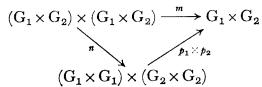
\includegraphics[keepaspectratio]{images/part002_baaabc67.jpg}}

其中 \(s(g, g') = (g', g)\)，\(m(g, g') = gg'\)，\(n(g, g') = g'g\)，这里 \(g\)、\(g'\) 取遍 \(G\)。这个图是交换的。因而 \(n_*(t \otimes t') = m_*(s_*(t \otimes t')) = m_*(t' \otimes t)\)。这个等式恰好就是 (i)。断言 (ii) 由 (i) 与命题 6 得出。

命题 8. 设 G、H 为李群，\(\phi\) 为 G 到 H 的态射。若 \(t \in \mathcal{T}^{(\infty)}(G)\)，则 \(\phi_{*}(t^{\vee}) = (\phi_{*}(t))^{\vee}\)。

设 \(\theta\)（相应地 \(\theta'\)）为 G 到 G（相应地 H 到 H）的映射 \(g \mapsto g^{-1}\)。于是 \(\phi \circ \theta = \theta' \circ \phi\)，从而 \(\phi_*(\theta_*(t)) = \theta'_*(\phi_*(t))\)。

命题 9. 设 \(\mathrm{G}_1, \cdots, \mathrm{G}_n\) 为李群，\(\mathrm{G} = \mathrm{G}_1 \times \cdots \times \mathrm{G}_n\)。若向量空间 \(\mathcal{T}^{(\infty)}(\mathrm{G})\) 与 \(\mathcal{T}^{(\infty)}(\mathrm{G}_1) \otimes \cdots \otimes \mathcal{T}^{(\infty)}(\mathrm{G}_n)\) 典范地认同，则代数 \(\mathcal{T}^{(\infty)}(\mathrm{G})\) 是诸代数 \(\mathcal{T}^{(\infty)}(\mathrm{G}_1), \ldots, \mathcal{T}^{(\infty)}(\mathrm{G}_n)\) 的张量积。若 \(t_i \in \mathcal{T}^{(\infty)}(\mathrm{G}_i)\)（\(i = 1, \ldots, n\)），则

\[
\left(t _ {1} \otimes \dots \otimes t _ {n}\right) ^ {\vee} = t _ {1} ^ {\vee} \otimes \dots \otimes t _ {n} ^ {\vee}.
\]

只需考虑 \(n = 2\) 的情形。设 \(t_1, t_1'\) 属于 \(\mathcal{T}^{(\infty)}(\mathrm{G}_1)\)，\(t_2, t_2'\) 属于 \(\mathcal{T}^{(\infty)}(\mathrm{G}_2)\)。我们需要证明 \((t_1 \otimes t_2) * (t_1' \otimes t_2') = (t_1 * t_1') \otimes (t_2 * t_2')\) 以及 \((t_1 \otimes t_2)^{\vee} = t_1^{\vee} \otimes t_2^{\vee}\)。考虑图

\pandocbounded{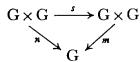
\includegraphics[keepaspectratio]{images/part002_69e6a490.jpg}}

其中 \(m((x_1, x_2), (x_1', x_2')) = (x_1x_1', x_2x_2')\)，

\[
n ((x _ {1}, x _ {2}), (x _ {1} ^ {\prime}, x _ {2} ^ {\prime})) = ((x _ {1}, x _ {1} ^ {\prime}), (x _ {2}, x _ {2} ^ {\prime})),
\]

\(p_1(x_1, x_1') = x_1x_1', p_2(x_2, x_2') = x_2x_2'\)。这个图是交换的。因而

\[
m _ {*} \left(\left(t _ {1} \otimes t _ {2}\right) \otimes \left(t _ {1} ^ {\prime} \otimes t _ {2} ^ {\prime}\right)\right) = \left(p _ {1} \otimes p _ {2}\right) _ {*} \left(n _ {*} \left(\left(t _ {1} \otimes t _ {2}\right) \otimes \left(t _ {1} ^ {\prime} \otimes t _ {2} ^ {\prime}\right)\right)\right),
\]

也就是

\[
\begin{array}{r l} (t _ {1} \otimes t _ {2}) * (t _ {1} ^ {\prime} \otimes t _ {2} ^ {\prime}) & = (p _ {1} \otimes p _ {2}) _ {*} ((t _ {1} \otimes t _ {1} ^ {\prime}) \otimes (t _ {2} \otimes t _ {2} ^ {\prime})) \\ & = p _ {1 *} (t _ {1} \otimes t _ {1} ^ {\prime}) \otimes p _ {2 *} (t _ {2} \otimes t _ {2} ^ {\prime}) \\ & = (t _ {1} * t _ {1} ^ {\prime}) \otimes (t _ {2} * t _ {2} ^ {\prime}). \end{array}
\]

同理可以看出 \((t_1\otimes t_2)^\vee = t_1^\vee \otimes t_2^\vee\)

命题 10. 设 H 为 G 的李子群，\(i: \mathrm{H} \to \mathrm{G}\) 为典范单射。于是 \(i_*\) 是代数 \(\mathcal{T}^{(\infty)}(\mathrm{H})\) 到代数 \(\mathcal{T}^{(\infty)}(\mathrm{G})\) 中的单射同态，且 \(i_*(t^\vee) = (i_*(t))^{\vee}\)（对所有 \(t \in \mathcal{T}^{(\infty)}(\mathrm{H})\)）。

这由命题 6、命题 8 以及 Differentiable and Analytic Manifolds, R, 13.2.3 得出。

\(\mathcal{T}^{(\infty)}(H)\) 借助命题 10 的同构与 \(\mathcal{T}^{(\infty)}(G)\) 的一个子代数认同。

注。若 H 是李拟子群，命题 10 仍然成立。

我们回忆 (Differentiable and Analytic Manifolds, R, 13.5.1)，若 V 是 K 上的解析流形，则 \(\mathcal{T}^{(\infty)}(\mathrm{V})\) 典范地具有一个带余单位的 K 上余代数结构；余单位是 \(\mathcal{T}^{(\infty)}(\mathrm{G})\) 到 K 中的线性映射，它把 \(\mathrm{T}_x^{(\infty)}(\mathrm{V})\) 的每个元素对应到其常数项。

命题 11. 设 G 为李群。

\begin{enumerate}
\def\labelenumi{(\roman{enumi})}
\item
  带卷积的余代数 \(\mathcal{T}^{(\infty)}(\mathbf{G})\) 是一个双代数 (Algebra, Chapter III, § 11, no. 4)。
\item
  设 \(c\) 为 \(\mathcal{T}^{(\infty)}(\mathbf{G})\) 上的余积。设 \(t \in \mathcal{T}^{(\infty)}(\mathbf{G})\)，并记
\end{enumerate}

\[
c (t) = \sum_ {i = 1} ^ {n} t _ {i} \otimes t _ {i} ^ {\prime}.
\]

于是 \(c(t^{\vee}) = \sum_{i=1}^{n} t_{i}^{\vee} \otimes t_{i}^{\prime\vee}\)。

我们证明 (i)。在所引的双代数定义中，条件 (1) 由命题 2 与命题 3 得出，条件 (2) 由 Differentiable and Analytic Manifolds, R, 13.5.1 得出。设 \(d\) 为映射 \(g \mapsto (g, g)\)（从 G 到 \(\mathrm{G} \times \mathrm{G}\)）。于是 \(c = d_{*}\)，因而 \(c\) 是代数态射（命题 6 与命题 9），这就是条件 (3)。设 \(t \in \mathrm{T}_{g}^{\infty}(\mathrm{G})\)、\(t' \in \mathrm{T}_{g'}^{\infty}(\mathrm{G})\) 都没有常数项，且 \(\lambda\)、\(\lambda'\) 是 K 的元素；于是 \(\varepsilon_{g} \otimes t'\)、\(t \otimes \varepsilon_{g'}\)、\(t \otimes t'\) 都没有常数项 (Differentiable and Analytic Manifolds, R, 13.4.1)，因而 \((\lambda\varepsilon_{g} + t) * (\lambda' \varepsilon_{g'} + t')\) 的常数项是 \(\lambda\lambda'\)；于是条件 (4) 成立。

我们证明 (ii)。由命题 8 与命题 9，

\[
c (t ^ {\vee}) = d _ {*} (t ^ {\vee}) = (d _ {*} (t)) ^ {\vee} = \left(\sum_ {i = 1} ^ {n} t _ {i} \otimes t _ {i} ^ {\prime}\right) ^ {\vee} = \sum_ {i = 1} ^ {n} t _ {i} ^ {\prime \vee} \otimes t _ {i} ^ {\vee}.
\]

命题 12. 设 G、H 为两个李群，\(\phi\) 为 G 到 H 的态射。于是 \(\phi_{*}\) 是 \(\mathcal{T}^{(\infty)}(G)\) 到 \(\mathcal{T}^{(\infty)}(H)\) 的双代数态射。

这由命题 6 与 Differentiable and Analytic Manifolds, R, 13.5.1 得出。

设 \(G\) 为李群。卷积与余积在 \(U(G)\) 上的限制在 \(U(G)\) 上定义了一个双代数结构。我们有 \(U(G)^{\vee} = U(G)\)。若 \(\phi: G \to H\) 是李群态射，我们用 \(U(\phi)\) 表示映射 \(t \mapsto \phi_{*}(t)\)（从 \(U(G)\) 到 \(U(H)\)）；它是一个双代数态射。若 \(\psi: H \to L\) 是另一个李群态射，则 \(U(\psi \circ \phi) = U(\psi) \circ U(\phi)\)。若 \(\phi\) 是浸入（相应地浸没），则由 Differentiable and Analytic Manifolds, R, 13.2.3，\(U(\phi)\) 是单射的（相应地满射的）。特别地，若 \(H\) 是 \(G\) 的李子群，则 \(U(H)\) 与 \(U(G)\) 的一个子代数认同，且 \(U(H)\) 上的余积是 \(U(G)\) 上余积的限制。若 \(H\) 在 \(G\) 中是开的，则 \(U(H) = U(G)\)。若 \(G_1, G_2\) 是李群，则 \(U(G_1 \times G_2)\) 与 \(U(G_1) \times U(G_2)\) 认同。\(U(G)\) 的本原元素就是 \(T_e(G)\) 的元素 (Differentiable and Analytic Manifolds, R, 13.5.3)。

再设 \(\phi: \mathrm{G} \to \mathrm{H}\) 为李群态射。若把 \(\operatorname{gr} \mathrm{U}(\mathrm{G})\) 与 \(\mathrm{TS}(\mathrm{T}_e(\mathrm{G}))\) 认同，把 \(\operatorname{gr} \mathrm{U}(\mathrm{H})\) 与 \(\mathrm{TS}(\mathrm{T}_e(\mathrm{H}))\) 认同，则 \(\operatorname{gr} \mathrm{U}(\phi)\) 与 \(\mathrm{TS}(\mathrm{T}_e(\phi))\) 认同 (Differentiable and Analytic Manifolds, R, 13.3.5)。我们把这一点应用于同构 \(g \mapsto g^{-1}\)（从 \(\mathrm{G}\) 到 \(\mathrm{G}^{\vee}\) 上）；这时 \(\mathrm{T}_e(\phi) = -1\)，因而

\[
t \in \mathrm{U} _ {s} (\mathrm{G}) \Rightarrow t ^ {\vee} \equiv (- 1) ^ {s} t \bmod \mathrm{U} _ {s - 1} (\mathrm{G}).\tag{3}
\]

\subsection{群在流形上作用的情形}

设 \(G\) 为李群，\(X\) 为 \(C^r\) 类流形，\(f\) 为一个 \(C^r\) 类的、\(G\) 在 \(X\) 上的左作用律。若 \(t \in T_g^{(s)}(G)\)、\(u \in T_x^{(s')}(\mathbf{X})\) 且 \(s + s' \leqslant r\)，我们用 \(t * u\) 表示 \(t \otimes u\) 在 \(f_*\) 下的像。我们把乘积 \(*\) 延拓为一个仍记作 * 的双线性映射，从 \(\mathcal{T}^{(s)}(G) \times \mathcal{T}^{(s')}(\mathbf{X})\) 到 \(\mathcal{T}^{(s+s')}(\mathbf{X})\)。第 1 节的命题 1 经过明显的修改便可推广到当前的情形。

当 G 通过左平移作用在它自身上时，我们便重新得到第 1 节的定义 1。

命题 13. 设 \(t \in \mathcal{T}^{(s)}(\mathbf{G})\)，\(t' \in \mathcal{T}^{(s')}(\mathbf{G})\)，\(u \in \mathcal{T}^{(s'')}(\mathbf{X})\)，满足

\[
s + s ^ {\prime} + s ^ {\prime \prime} \leqslant r.
\]

则 \((t*t')*u=t*(t'*u)\)。

这可以像第 1 节的命题 2 那样证明。

特别地，若 \(r \leqslant \infty\)，则向量空间 \(\mathcal{T}^{(\infty)}(\mathbf{X})\) 是代数 \(\mathcal{T}^{(\infty)}(\mathbf{G})\)（带乘积 \(*\)）上的一个左模。

命题 14. (i) 设 \(g_0 \in G\)，\(\tau(g_0)\) 为映射 \(x \mapsto f(g_0, x)\)（从 \(X\) 到 \(X\)）。若 \(u \in \mathcal{T}^{(r)}(X)\)，则 \(\tau(g_0)_*u = \varepsilon_{g_0} * u\)。

\begin{enumerate}
\def\labelenumi{(\roman{enumi})}
\setcounter{enumi}{1}
\tightlist
\item
  设 \(x_0 \in \mathbf{X}\)，\(\rho(x_0)\) 为映射 \(g \mapsto f(g, x_0)\)（从 \(G\) 到 \(X\)）。若 \(t \in T^{(r)}(G)\)，则 \(\rho(x_0)_*t = t * \varepsilon_{x_0}\)。
\end{enumerate}

这可以像第 1 节的命题 3 那样证明。

特别地，若 \(u \in \mathrm{T}(\mathrm{X})\) 且 \(t \in \mathrm{T}(\mathrm{G})\)，则 \(\varepsilon_{g_0} * u\) 与 \(t * \varepsilon_{x_0}\) 分别等于 § 2 第 2 节中定义的乘积 \(g_0u\) 与 \(tx_0\)。

命题 15. 设 G（相应地 G'）为李群，X（相应地 X'）为 \(C^{r}\) 类流形。设给定了 G（相应地 G'）在 X（相应地 X'）上的一个 \(C^{r}\) 类左作用律。设 \(\phi\) 为 G 到 G' 的态射，\(\psi\) 为 X 到 X' 的一个 \(\phi\)-态射。设 \(t \in \mathcal{T}^{(s)}(G)\)、\(u \in \mathrm{T}^{(s')}(\mathrm{X})\) 满足 \(s + s' \leqslant r\)。则

\[
\psi_ {*} (t * u) = \phi_ {*} (t) * \psi_ {*} (u).
\]

这可以像第 2 节的命题 6 那样证明。

注。设 \(f\) 为一个 \(\mathbf{C}^r\) 类的、\(\mathbf{G}\) 在 \(\mathbf{X}\) 上的右作用律。若 \(t \in \mathcal{T}^{(s)}(\mathbf{G})\)、\(u \in \mathcal{T}^{(s')}(\mathbf{X})\) 且 \(s + s' \leqslant r\)，我们用 \(u * t\) 表示 \(u \otimes t\) 在 \(f_*\) 下的像。命题 13、14、15 以明显的方式移植到这一情形。

命题 16. 设 G、G' 为李群，X 为 \(C^{r}\) 类流形，且设 G（相应地 G'）在 X 上左作用（相应地右作用），使得 \((gx)g' = g(xg')\) 对所有 \(x \in X\)、\(g \in G\)、\(g' \in G'\) 成立。设 \(t \in \mathcal{T}^{(s)}(G)\)、\(t' \in \mathcal{T}^{(s')}(\mathrm{G}')\)、\(t'' \in \mathrm{T}^{(s'')}(\mathrm{X})\) 满足 \(s + s' + s'' \leqslant r\)。则

\[
(t * t ^ {\prime \prime}) * t ^ {\prime} = t * (t ^ {\prime \prime} * t ^ {\prime}).
\]

\((t*t'')*t'\)（相应地 \(t*(t''*t')\)）是 \(t\otimes t''\otimes t'\) 在 G × X × G' 到 X 的映射 \((g,x,g')\mapsto(gx)g'\)（相应地 \(g(xg')\)）下的像。

\subsection{点分布与函数的卷积}

设 G 为李群，X 为 \(C^{r}\) 类流形，\((g, x) \mapsto gx\) 为 G 在 X 上的一个 \(C^{r}\) 类左作用律。对所有 \(x \in X\)，用 \(\rho(x)\) 表示 x 的轨道映射。

定义 3. 设 \(t \in \mathcal{T}^{(s)}(\mathrm{G})\)，\(s \leqslant r\)。设 \(f: \mathrm{X} \to \mathrm{F}\) 为取值于一个分离多范空间的 \(\mathbf{C}^r\) 类函数（例如 \(\mathrm{F} = \mathrm{K}\)）。\(t\) 与 \(f\) 的卷积，记作 \(t * f\)，是 \(\mathbf{X}\) 上以 \(\mathrm{F}\) 为值域、由

\[
(t * f) (x) = \langle t ^ {\vee} * \varepsilon_ {x}, f \rangle .
\]

于是

\[
\begin{array}{l l} (t * f) (x) = \langle \rho (x) _ {*} (t ^ {\vee}), f \rangle & (\text {no. 3, Proposition 14 (ii)}) \\ = \langle t ^ {\vee}, f \circ \rho (x) \rangle & (Diff. \& Anal. Man., R, 13.2.3) \\ = \langle t, (f \circ \rho (x)) ^ {\vee} \rangle & (Diff. \& Anal. Man., R, 13.2.3). \end{array}\tag{4}
\]

注意，定义 3 也可以写成更对称的形式

\[
\langle \varepsilon_ {x}, t * f \rangle = \langle t ^ {\vee} * \varepsilon_ {x}, f \rangle .\tag{5}
\]

函数 \((g,x)\mapsto f(gx) = (f\circ \rho (x))(g)\)（\(\mathbf{G}\times \mathbf{X}\) 上的）是 \(\mathbf{C}^r\) 类的。由 Differentiable and Analytic Manifolds, R, 13.4.4，函数 \(x\mapsto \langle t^\vee,f\circ \rho (x)\rangle\) 因而是 \(\mathbf{C}^{r - s}\) 类的（若 \(s < \infty\)）。换句话说，若 \(s < \infty\)，则 \(t*f\) 是 \(\mathbf{C}^{r - s}\) 类的。

显然，\(t * f\) 线性地依赖于 \(t\) 和 \(f\)。

特别地，公式 (4) 蕴含：对 \(g \in G\)，

\[
\left(\varepsilon_ {g} * f\right) (x) = f \left(g ^ {- 1} x\right)\tag{6}
\]

也就是

\begin{enumerate}
\def\labelenumi{(\arabic{enumi})}
\setcounter{enumi}{6}
\tightlist
\item
\end{enumerate}

\[
\varepsilon_ {g} * f = \gamma (g) f.
\]

设 \(\mathbf{K} = \mathbf{R}\) 或 \(\mathbf{C}\)，\(\mathbf{G}\) 与 \(\mathbf{X}\) 都是有限维的，且 \(\mathbf{X}\) 具有一个在 \(\mathbf{G}\) 下不变的正测度。\(\varepsilon_g * f\) 的定义与 Integration, Chapter VIII, § 4, no. 1 中的定义一致（参看~同处公式 (2)）。

命题 17. 设 \(t \in \mathcal{T}^{(s)}(\mathrm{G})\)，\(t' \in \mathcal{T}^{(s')}(\mathrm{X})\)，\(f: X \to \mathrm{F}\) 为 \(\mathbf{C}^{r}\) 类函数，满足 \(s + s' \leqslant r\)。则

\[
\langle t ^ {\prime}, t * f \rangle = \langle t ^ {\vee} * t ^ {\prime}, f \rangle .
\]

\[
\begin{array}{l l} \langle t ^ {\prime}, t * f \rangle = \langle t ^ {\prime}, x \mapsto \langle t, g \mapsto f (g ^ {- 1} x) \rangle \rangle & \text { by   (4) } \\ = \langle t \otimes t ^ {\prime}, (g, x) \mapsto f (g ^ {- 1} x) \rangle & \text {(Diff. \& Anal. Man., R, 13.4.4)} \\ = \langle t ^ {\vee} \otimes t ^ {\prime}, (g, x) \mapsto f (g x) \rangle & \text {(Diff. \& Anal. Man., R, 13.2.3)} \\ = \langle t ^ {\vee} * t ^ {\prime}, f \rangle . \end{array}
\]

命题 18. 设 \(t \in \mathcal{T}^{(s)}(\mathrm{G})\)，\(t' \in \mathcal{T}^{(s')}(\mathrm{G})\)，\(f: \mathrm{X} \to \mathrm{F}\) 为 \(\mathbf{C}^r\) 类函数，满足 \(s + s' \leqslant r\)。则

\[
(t * t ^ {\prime}) * f = t * (t ^ {\prime} * f).
\]

对所有 \(x \in X\)，

\[
\begin{array}{l l} \langle \varepsilon_ {x}, (t * t ^ {\prime}) * f \rangle = \langle (t * t ^ {\prime}) ^ {\vee} * \varepsilon_ {x}, f \rangle & \text {by (5)} \\ = \langle t ^ {\prime \vee} * (t ^ {\vee} * \varepsilon_ {x}), f \rangle & \text {(Propositions 2 and 7)} \\ = \langle t ^ {\vee} * \varepsilon_ {x}, t ^ {\prime} * f \rangle & \text {(Proposition 17)} \\ = \langle \varepsilon_ {x}, t * (t ^ {\prime} * f) \rangle & \text {(Proposition 17).} \end{array}
\]

若 \(r \geqslant \infty\)，则我们看到，\(C^\infty\) 类函数（\(X\) 上、以 \(F\) 为值域）的集合是代数 \(\mathcal{T}^{(\infty)}(G)\) 上的一个左模。

命题 19. 设 \(t \in \mathcal{T}^{(s)}(\mathrm{G})\)，\(s \leqslant r\)。设 \(f\)（相应地 \(f'\)）为 \(\mathrm{C}^r\) 类函数，定义在 \(\mathbf{X}\) 上、取值于一个分离多范空间 \(\mathrm{F}\)（相应地 \(\mathrm{F}'\)）。设 \((u, u') \mapsto uu'\) 为 \(\mathrm{F} \times \mathrm{F}'\) 到一个分离多范空间 \(\mathrm{F}''\) 中的连续双线性映射，使得 \(ff'\) 是 \(\mathrm{C}^r\) 类函数，定义在 \(\mathbf{X}\) 上、取值于 \(\mathrm{F}''\)。设 \(\sum_{i=1}^{n} t_i \otimes t_i'\) 为 \(t\) 在余积下在 \(\mathcal{T}^{(s)}(\mathrm{G}) \otimes \mathcal{T}^{(s)}(\mathrm{G})\) 中的像。则

\[
t * (f f ^ {\prime}) = \sum_ {i = 1} ^ {n} (t _ {i} * f) (t _ {i} ^ {\prime} * f ^ {\prime}).
\]

设 \(x \in X\)，并用 \(\rho(x)\) 表示 x 的轨道映射。于是

\[
\begin{array}{l l} \langle \varepsilon_ {x}, t * (f f ^ {\prime}) \rangle = \langle t ^ {\vee}, (f f ^ {\prime}) \circ \rho (x) \rangle & \text {by (4)} \\ = \langle t ^ {\vee}, (f \circ \rho (x)) (f ^ {\prime} \circ \rho (x)) \rangle \\ = \sum_ {i = 1} ^ {n} \langle t _ {i} ^ {\vee}, f \circ \rho (x) \rangle \langle t _ {i} ^ {\prime \vee}, f ^ {\prime} \circ \rho (x) \rangle \\ & (\text {Diff. \& Man. Anal., R, 13.5.2}) \\ = \sum_ {i = 1} ^ {n} \langle \varepsilon_ {x}, t _ {i} * f \rangle \langle \varepsilon_ {x}, t _ {i} ^ {\prime} * f ^ {\prime} \rangle & \text {by (4).} \end{array}
\]

注 1. 设 G 为李群，X 为 \(\mathbf{C}^r\) 类流形，\((x,g)\mapsto xg\) 为 G 在 X 上的一个 \(\mathbf{C}^r\) 类右作用律。若 \(t\in \mathcal{T}^{(s)}(\mathrm{G})\)（\(s\leqslant r\)）且 \(f\colon \mathrm{X}\to \mathrm{F}\) 是 X 上的一个 \(\mathbf{C}^r\) 类函数，我们用 \(f*t\) 表示 X 上由

\[
\begin{array}{r l} \langle \varepsilon_ {x}, f * t \rangle & = \langle \varepsilon_ {x} * t ^ {\vee}, f \rangle \\ & = \langle \rho (x) _ {*} (t ^ {\vee}), f \rangle \\ & = \langle t ^ {\vee}, f \circ \rho (x) \rangle \\ & = \langle t, (f \circ \rho (x)) ^ {\vee} \rangle . \end{array}\tag{8}
\]

特别地

\[
(f * \varepsilon_ {g}) (x) = f (x g ^ {- 1})\tag{9}
\]

也就是

\[
f * \varepsilon_ {g} = \delta (g) ^ {- 1} f.\tag{10}
\]

在明显的记号下，命题 17、18、19 成为

\begin{enumerate}
\def\labelenumi{(\arabic{enumi})}
\setcounter{enumi}{10}
\tightlist
\item
\end{enumerate}

\[
\langle t ^ {\prime}, f * t \rangle = \langle t ^ {\prime} * t ^ {\vee}, f \rangle\tag{11}
\]

\[
f * (t * t ^ {\prime}) = (f * t) * t ^ {\prime}\tag{12}
\]

\[
(f f ^ {\prime}) * t = \sum_ {i = 1} ^ {n} (f * t _ {i}) (f ^ {\prime} * t _ {i} ^ {\prime}).\tag{13}
\]

命题 20. 设 \(G\)、\(G'\) 为李群，\(X\) 为 \(C^r\) 类流形，\((g, x) \mapsto gx\)（相应地 \((x, g') \mapsto xg'\)）为 \(C^r\) 类的、\(G\)（相应地 \(G'\)）在 \(X\) 上的左（相应地右）作用律。设 \((gx)g' = g(xg')\) 对所有 \(x \in X\)、\(g \in G\)、\(g' \in G'\) 成立。设 \(t \in \mathcal{T}^{(s)}(G)\)、\(t' \in \mathcal{T}^{(s')}(\mathrm{G}')\) 且 \(f: X \to F\) 为 \(C^r\) 类函数，满足 \(s + s' \leqslant r\)。则

\[
(t * f) * t ^ {\prime} = t * (f * t ^ {\prime}).
\]

对所有 \(x \in X\)，

\[
\begin{array}{l l} \langle \varepsilon_ {x}, (t * f) * t ^ {\prime} \rangle = \langle \varepsilon_ {x} * t ^ {\prime \vee}, t * f \rangle & \text { by   (8) } \\ = \langle t ^ {\vee} * (\varepsilon_ {x} * t ^ {\prime \vee}), f \rangle & \text {(Proposition 17)} \\ = \langle t ^ {\vee} * \varepsilon_ {x}, f * t ^ {\prime} \rangle & \text {(Proposition 2 and (11))} \\ = \langle \varepsilon_ {x}, t * (f * t ^ {\prime}) \rangle & \text { by   (5). } \end{array}
\]

特别地，把 G 看作通过左平移和右平移作用在它自身上。若 \(f \colon \mathbf{G} \to \mathbf{F}\) 是 G 上的 \(\mathbf{C}^r\) 类函数且 \(t \in \mathcal{T}^{(s)}(\mathbf{G})\)（\(s \leqslant r\)），则 \(t * f\) 与 \(f * t\) 当 \(s < \infty\) 时是 G 上的 \(\mathbf{C}^{r - s}\) 类函数。进而，设 \(t' \in \mathcal{T}^{(s')}(\mathbf{G})\) 满足 \(s + s' \leqslant r\)。则

\[
(t * f) * t ^ {\prime} = t * (f * t ^ {\prime}).\tag{14}
\]

特别地，\(\mathcal{C}^{\infty}(\mathrm{G})\) 是一个 \((\mathcal{T}^{(\infty)}(\mathrm{G}),\mathcal{T}^{(\infty)}(\mathrm{G}))\)-双模。公式 (5) 与 (8) 的特殊情形是

\[
\langle t, f \rangle = \left\langle \varepsilon_ {e}, t ^ {\vee} * f \right\rangle = \left\langle \varepsilon_ {e}, f * t ^ {\vee} \right\rangle .\tag{15}
\]

注 2. 设 \((g,x)\mapsto gx\) 为一个 \(\mathbf{C}^r\) 类的、\(G\) 在 \(X\) 上的左作用律。设 \(t\in \mathbf{U}_s(\mathbf{G})\)（\(s\leqslant r\)），\(\Omega\) 为 \(X\) 的开子集，\(f\colon \Omega \to F\) 为 \(\mathbf{C}^r\) 类函数。\(t*f\) 也可以由公式 (4) 或 (5) 来定义；它是定义在 \(\Omega\) 上、取值于 \(F\) 的函数，是 \(\mathbf{C}^{r - s}\) 类的（若 \(s < \infty\)）。本节的结果以明显的方式推广到这一情形。

\subsection{由群在流形上的作用所定义的点分布场}

设 \((g,x)\mapsto\lambda(g,x)=gx\) 为 G 在 X 上的一个 \(C^{r}\) 类左作用律。设 \(s\leqslant r\) 且 \(t\in U_{s}(G)\)。对所有 \(x\in X\)，有 \(t*\varepsilon_{x}\in T_{x}^{(s)}(X)\)。映射 \(x\mapsto t*\varepsilon_{x}\) 称为由 t 及 G 在 X 上的作用所定义的点分布场，有时记作 \(D_{t}^{\lambda}\) 或简记作 \(D_{t}\)。设 \(\Omega\) 为 X 的开子集，F 为分离多范空间。若 \(f\colon\Omega\to F\) 是 \(C^{r}\) 类的且 \(s\leqslant r\)，则函数 \(t^{\vee}\ast f\)（\(\Omega\) 上的）也记作 \(D_{t}.f\)。于是

\[
(D _ {t} f) (x) = \langle t * \varepsilon_ {x}, f \rangle .\tag{16}
\]

若 \(s < \infty\)，则由第 4 节，\(D_t f \in \mathcal{C}^{r-s}(\Omega, F)\)。这样，\(f \mapsto D_t f\) 是 \(\mathcal{C}^r(\Omega, F)\) 到 \(\mathcal{C}^{r-s}(\Omega, F)\) 的映射（由于记号的滥用，常记作 \(D_t\)）。

若 \(t \in \mathrm{U}_s(\mathrm{G})\)、\(t' \in \mathrm{U}_{s'}(\mathrm{G})\) 且 \(s + s' \leqslant r\)，则由第 4 节的命题 18，

\[
\mathrm{D} _ {t * t ^ {\prime}} f = \mathrm{D} _ {t ^ {\prime}} (\mathrm{D} _ {t} f)\tag{17}
\]

因而，利用上面指出的记号滥用，有

\[
\mathrm{D} _ {t * t ^ {\prime}} = \mathrm{D} _ {t ^ {\prime}} \circ \mathrm{D} _ {t}.\tag{18}
\]

设 G 与 X 都是有限维的。映射 \((t, x) \mapsto t \otimes \varepsilon_{x}\)（从 \(\mathrm{T}^{(\mathrm{s})}(\mathrm{G}) \times \mathrm{X}\) 到向量丛 \(\mathrm{T}^{(\mathrm{s})}(\mathrm{G} \times \mathrm{X})\)，cf.~Differentiable and Analytic Manifolds, R, 13.2.5）是 \(C^{r-s}\) 类的。因而 (Differentiable and Analytic Manifolds, R, 13.2.5)，映射 \((t, x) \mapsto t * \varepsilon_{x}\)（从 \(\mathrm{T}^{(\mathrm{s})}(\mathrm{G}) \times \mathrm{X}\) 到向量丛 \(\mathrm{T}^{(\mathrm{s})}(\mathrm{X})\)）是 \(C^{r-s}\) 类的。特别地，\(D_{t}\) 是 Differentiable and Analytic Manifolds, R, 14.1.6 意义下阶数 \(\leqslant s\) 且类为 \(C^{r-s}\) 的微分算子。由公式 (16)，函数 \(D_{t}f\) 就是 f 在这个微分算子下的像 (Differentiable and Analytic Manifolds, R, 14.1.4)。

我们现在不再假设 G 与 X 都是有限维的。设 \(\psi\) 为流形 X 的自同构，\(\Delta\) 为 X 上的一个点分布场。按照一般的定义，\(\Delta\) 在 \(\psi\) 下的变换是 X 上的这样一个点分布场：它在 \(\psi(x)\) 的值是 \(\psi_{*}(\Delta(x))\)；我们把这个映射记作 \(\psi(\Delta)\)。若 \(g \in G\) 且 \(\tau(g)\) 表示 X 的自同构 \(x \mapsto gx\)，则 \(\Delta\) 在 \(\tau(g)\) 下的变换也称为 \(\Delta\) 在 g 下的变换。

命题 21. 设 \(\psi\) 为与 G 的作用交换的 X 的自同构。则 \(D_{t}\) 在 \(\psi\) 下不变。

对所有 \(x \in X\)，

\[
\begin{array}{r l} (\psi (\mathrm{D} _ {t})) (\psi (x)) & = \psi_ {*} (\mathrm{D} _ {t} (x)) = \psi_ {*} (t * \varepsilon_ {x}) \\ & = t * \psi_ {*} (\varepsilon_ {x}) \quad \text {(Proposition 15)} \\ & = t * \varepsilon_ {\psi (x)} = \mathrm{D} _ {t} (\psi (x)). \end{array}
\]

命题 22. 若 \(g \in G\)，则 \(D_t\) 在 \(g\) 下的变换是 \(D_{\varepsilon_g * t * \varepsilon_{g^{-1}}}\)。

这个变换在 gx 处的值是

\[
\begin{array}{r l r} \tau (g) _ {*} (\mathrm{D} _ {t} (x)) & = \tau (g) _ {*} (t * \varepsilon_ {x}) \\ & = \varepsilon_ {g} * (t * \varepsilon_ {x}) & \text {(Proposition 14 (i))} \\ & = (\varepsilon_ {g} * t * \varepsilon_ {g^{-1}}) * \varepsilon_ {g x} & \text {(Propositions 1 and 2)} \\ & = \mathrm{D} _ {\varepsilon_ {g} * t * \varepsilon_ {g^{-1}}} (g x). \end{array}
\]

设 \((x,g)\mapsto \mu (x,g) = xg\) 为 G 在 X 上的一个 \(\mathbf{C}^r\) 类右作用律。设 \(s\leqslant r\) 且 \(t\in \mathrm{U}_{s}(\mathrm{G})\)。对所有 \(x\in \mathbf{X}\)，有 \(\varepsilon_{x}*t\in \mathrm{T}_{x}^{(s)}(\mathbf{X})\)。映射 \(x\mapsto \varepsilon_x*t\) 称为由 \(t\) 及 G 在 X 上的作用所定义的分布场，有时记作 \(\mathrm{D}_{t}^{\mu}\) 或简记作 \(\mathrm{D}_t\)。设 \(\Omega\) 为 X 的开子集。若 \(f:\Omega \to F\) 是 \(\mathbf{C}^r\) 类的，则函数 \(f*t^{\vee}\) 记作 \(\mathrm{D}_t f\)。于是

\[
\left(\mathrm{D} _ {t} f\right) (x) = \langle \varepsilon_ {x} * t, f \rangle\tag{19}
\]

且在明显的记号下，有

\begin{enumerate}
\def\labelenumi{(\arabic{enumi})}
\setcounter{enumi}{19}
\tightlist
\item
\end{enumerate}

\[
D _ {t * t ^ {\prime}} f = \mathrm{D} _ {t} (\mathrm{D} _ {t ^ {\prime}} f)\tag{20}
\]

\[
\mathrm{D} _ {t * t ^ {\prime}} = \mathrm{D} _ {t} \circ \mathrm{D} _ {t ^ {\prime}}\tag{21}.
\]

命题 21 仍然成立。设 \(g \in G\)。\(D_t\) 在 \(g\) 下的变换（即在自同构 \(x \mapsto xg\)（\(X\) 的自同构）下的变换）是 \(D_{\varepsilon_{g^{-1}} * t * \varepsilon_g}\)。

\subsection{李群上的不变点分布场}

定义 4. 设 G 为李群。G 上的一个分布场若在 G 的左（相应地右）平移下不变，则称为左不变的（相应地右不变的）。

换句话说，分布场 \(g \mapsto \Delta_g\)（\(G\) 上的）是左不变的，如果

\[
\Delta_ {g g ^ {\prime}} = \gamma (g) _ {*} \Delta_ {g ^ {\prime}} \quad \text { for } g, g ^ {\prime} \text { in } G,
\]

或者等价地，如果

\[
\Delta_ {g g ^ {\prime}} = \varepsilon_ {g} * \Delta_ {g ^ {\prime}} \quad \text { for   } g, g ^ {\prime} \text {   in   G. }
\]

它是右不变的，如果

\[
\Delta_ {g g ^ {\prime}} = \delta (g ^ {\prime - 1}) _ {*} \Delta_ {g} \quad \text { for   } g, g ^ {\prime} \text {   in   G },
\]

或者等价地，如果.

\[
\Delta_ {g g ^ {\prime}} = \Delta_ {g} * \varepsilon_ {g ^ {\prime}}, \quad \text { for   } g, g ^ {\prime} \text {   in   G. }
\]

定义 5. 设 G 为李群，\(t \in \mathrm{U}(\mathrm{G})\)。用 \(\mathbf{L}_t\) 表示 G 上的分布场 \(g \mapsto \varepsilon_g * t\)，用 \(\mathbb{R}_t\) 表示 G 上的分布场 \(g \mapsto t * \varepsilon_g\)。

换句话说，\(L_{t}\)（相应地 \(R_{t}\)）是由 t 与借助映射 \((g, g') \mapsto gg'\) 在 G 上右（相应地左）作用的 G 所定义的分布场。设 \(\Omega\) 为 G 的开子集，F 为分离多范空间；若 \(f \in \mathcal{C}^{\omega}(\Omega, \mathrm{F})\)，则 \(\mathrm{L}_{t}f = f * t^{\vee} \in \mathcal{C}^{\omega}(\Omega, \mathrm{F})\)，且

\[
\mathrm{R} _ {t} f = t ^ {\vee} * f \in \mathcal {C} ^ {\omega} (\Omega , \mathrm{F})
\]

（第 5 节）。若 G 是有限维的，则微分算子 \(L_{t}\) 与 \(R_{t}\) 是 \(C^{\omega}\) 类的（第 5 节）。

命题 23. (i) 映射 \(t \mapsto \mathbf{L}_t\)（相应地 \(t \mapsto \mathbf{R}_t\)）是向量空间 \(\mathbf{U}(\mathbf{G})\) 到 \(\mathbf{G}\) 上左（相应地右）不变分布所成的向量空间上的同构。

\begin{enumerate}
\def\labelenumi{(\roman{enumi})}
\setcounter{enumi}{1}
\item
  对 U(G) 中的 \(t, t'\)，有 \(L_{t*t'} = L_t \circ L_{t'}\)，\(R_{t*t'} = R_{t'} \circ R_t\)，\(L_t \circ R_{t'} = R_{t'} \circ L_t\)（带有第 5 节的记号滥用）。
\item
  若 \(\theta\) 是映射 \(g \mapsto g^{-1}\)（从 \(\mathbf{G}\) 到 \(\mathbf{G}\) 上），则 \(\theta(\mathbf{L}_t) = \mathbf{R}_{t^{\vee}}\)。
\item
  若 \(t \in \mathrm{U}(\mathrm{G})\) 且 \(g \in \mathrm{G}\)，则 \((\mathrm{L}_t)_g = (\mathrm{R}_{\varepsilon_g * t * \varepsilon_{g^{-1}}})_g\)。
\end{enumerate}

在 G 中，每个右平移与每个左平移交换。于是由第 5 节的命题 21，\(L_{t}\) 是左不变的。由于 \((\mathbf{L}_{t})_{e}=t\)，映射 \(t\mapsto L_{t}\) 是单射的。设 \(\Delta\) 为 G 上的左不变分布场；设 \(t=\Delta_{e}\)；于是 \(\Delta\) 与 \(L_{t}\) 在 e 处有相同的值且都是左不变的，因而 \(\Delta=L_{t}\)。这就对 \(L_{t}\) 证明了 (i)，而对 \(R_{t}\) 的论证是类似的。公式 \(L_{t*t^{\prime}}=L_{t}\circ L_{t^{\prime}}\) 与 \(R_{t*t^{\prime}}=R_{t^{\prime}}\circ R_{t}\) 由 (21) 与 (18) 得出。设 \(t\in\mathrm{U}_{s}(\mathrm{G})\)、\(t^{\prime}\in\mathrm{U}_{s^{\prime}}(\mathrm{G}), f\in\mathcal{C}^{r}(\Omega,\mathrm{F})\)，其中 \(\Omega\) 是 G 中的开集且 \(s+s^{\prime}\leqslant r\)；于是

\[
\begin{array}{r l} \mathrm{L} _ {t} \mathrm{R} _ {t ^ {\prime}} f & = \mathrm{L} _ {t} (t ^ {\prime^ {\vee}} * f) = (t ^ {\prime^ {\vee}} * f) * t \\ & = t ^ {\prime^ {\vee}} * (f * t ^ {\vee}) \quad \text {(Proposition 20)} \\ & = \mathrm{R} _ {t ^ {\prime}} \mathrm{L} _ {t} f \end{array}
\]

因而 \(\mathbf{L}_t\circ \mathbf{R}_{t'} = \mathbf{R}_{t'}\circ \mathbf{L}_t\)。由于 \(\theta\) 是 \(\mathbf{G}\) 到 \(\mathbf{G}^{\vee}\) 的同构，\(\theta (\mathrm{L}_t)\) 是 \(\mathbf{G}\) 上的一个右不变分布场；它在 \(e\) 处的值是 \(\theta^{*}(t) = t^{\vee}\)，因而 \(\theta (\mathrm{L}_t) = \mathrm{R}_{t^{\vee}}\)。最后，

\[
\left(\mathrm{L} _ {t}\right) _ {g} = \varepsilon_ {g} * t = \left(\varepsilon_ {g} * t * \varepsilon_ {g^{-1}}\right) * \varepsilon_ {g} = \left(\mathrm{R} _ {\varepsilon_ {g} * t * \varepsilon_ {g^{-1}}}\right) _ {g}.
\]

注 1. 正是 G 通过右平移在它自身上的作用定义了左不变分布场。

注 2. 设 G 是有限维的。映射

\[
(t, g) \mapsto (\mathbf {R} _ {t}) _ {g} = t * \varepsilon_ {g}
\]

（从 \(\mathrm{U}_{s}(\mathrm{G})\times\mathrm{G}\) 到 \(\mathrm{T}^{(s)}(\mathrm{G})\)）是解析向量丛的同构；因为这个映射是双射的、在每个纤维上是线性的且是解析的（第 5 节）；另一方面，设 \(\phi:\mathrm{T}^{(s)}(\mathrm{G})\to\mathrm{U}_{s}(\mathrm{G})\times\mathrm{G}\) 为其逆双射；若 \(t\in\mathrm{T}_{g}^{(s)}(\mathrm{G})\)，则 \(\phi(t)=(t*\varepsilon_{g^{-1}},g)\)，因而 \(\phi\) 是解析的。同构 \(\phi\) 称为 \(\mathrm{T}^{(s)}(\mathrm{G})\) 的右平凡化。类似地，考虑映射 \((t,g)\mapsto(\mathrm{L}_{\mathrm{t}})_{g}=\varepsilon_{g}*t\)（从 \(\mathrm{U}_{s}(\mathrm{G})\times\mathrm{G}\) 到 \(\mathrm{T}^{(s)}(\mathrm{G})\)）；其逆同构称为 \(\mathrm{T}^{(s)}(\mathrm{G})\) 的左平凡化。通过限制，我们重新得到 \(\mathrm{T}(\mathrm{G})\) 的右平凡化和左平凡化 (§2, 第 2 节)。

\subsection{李群的李代数}

设 \(\mathbf{G}\) 为李群。在 \(\mathrm{U}(\mathbf{G})\) 中，如同在任何结合代数中一样，我们记 \([t, t'] = t * t' - t' * t\)。由于 \(\mathrm{T}_{e}(\mathbf{G})\) 是 \(\mathrm{U}(\mathbf{G})\) 的本原元素之集，有 \([\mathrm{T}_{e}(\mathbf{G}), \mathrm{T}_{e}(\mathbf{G})] \subset \mathrm{T}_{e}(\mathbf{G})\) (Chapter II, § 1, no. 2, Proposition 4)。因此，括号在 \(\mathrm{T}_{e}(\mathbf{G})\) 上的限制在 \(\mathrm{T}_{e}(\mathbf{G})\) 上定义了一个李代数结构。

引理 1. 设 \(\mathbf{X}\) 与 \(\mathbf{X}'\) 为完备可赋范空间，\(\mathbf{X}_0\) 为 \(\mathbf{X}\) 中 0 的开邻域，\(f\) 为 \(\mathbf{X}_0\) 到 \(\mathbf{X}'\) 的解析映射且满足 \(f(0) = 0\)。设 \(f = f_1 + f_2 + f_3 + \dots\) 为 \(f\) 在 0 处的幂级数展开，其中 \(f_i\) 是 \(i\) 次齐次连续多项式，定义在 \(\mathbf{X}\) 上、取值于 \(\mathbf{X}'\)。设 \(t\) 为 \(\mathrm{TS}^2 (\mathbf{X})\) 的元素，把它看作 \(\mathbf{X}\) 上支集含于 \(\{0\}\) 的点分布。设 \(t' = f_{\star}(t) \in \mathrm{TS}(\mathbf{X}')\)。\(t'\) 的 1 次齐次分量是 \(\langle f_2, t \rangle\)。

设 \(t_{1}^{\prime}\) 为这个分量。于是，对 \(X^{\prime}\) 到一个多范空间中的每个连续线性映射 u，

\[
\begin{array}{l l} u (t _ {1} ^ {\prime}) = \langle t ^ {\prime}, u \rangle & \text { because   } u \text {   is   continuous   and   linear } \\ = \langle t, u \circ f \rangle & (\text { Diff.   \&   Anal.   Man.,   R,   13.2.3 }) \\ = \langle t, u \circ f _ {2} \rangle & \text { because   } t \in \mathsf {T S} ^ {2} (\mathbf {X}) \\ = u (\langle t, f _ {2} \rangle) & (\text { Diff.   \&   Anal.   Man.,   R,   13.2.2 }), \end{array}
\]

引理由此得证。

命题 24. 设 G 为李群，(U, \(\phi\) , E) 为 G 上满足 \(\phi(e) = 0\) 的卡。设 \(e\) 的开邻域 V 满足 \(\mathrm{V}^2 \subset \mathrm{U}\)。设 \(m\) 为解析映射 \((a, b) \mapsto \phi(\phi^{-1}(a)\phi^{-1}(b))\)（从 \(\phi(V) \times \phi(V)\) 到 E 中）。设

\[
m = \sum_ {i, j \geqslant 0} m _ {i, j}
\]

为 \(m\) 在 \((0,0)\) 处的幂级数展开，其中 \(m_{i,j}\) 是双次数 \((i,j)\) 的、\(\mathbf{E} \times \mathbf{E}\) 上取值于 \(\mathbf{E}\) 的双齐次连续多项式。

\begin{enumerate}
\def\labelenumi{(\roman{enumi})}
\item
  \(m_{i,0} = m_{0,j} = 0\)（对所有 \(i \neq 1\) 与 \(j \neq 1\)）。
\item
  \(m_{1,0}(a,b)=a\) 且 \(m_{0,1}(a,b)=b\)（对所有 \(a\in E\)、\(b\in E\)）。
\item
  设 \(\psi: \mathrm{T}_e(\mathrm{G}) \to \mathrm{E}\) 为 \(\phi\) 在 \(e\) 处的微分。对所有 \(u, v\)（\(\mathrm{T}_e(\mathrm{G})\) 中的元素），
\end{enumerate}

\[
\psi ([ u, v ]) = m _ {1, 1} (\psi (u), \psi (v)) - m _ {1, 1} (\psi (v), \psi (u)).
\]

\(m(a,0) = a\)，\(m(0,b) = b\)（对所有 \(a\)、\(b\)，\(\phi (\mathrm{V})\) 中的元素），这就证明了 (i) 与 (ii)。设 \(u, v\) 属于 \(\mathrm{T_e(G)}\)。把 \(\mathrm{T_0(E)}\) 与 E 认同，从而把 \(\psi\) 与 \(\mathrm{T_e}(\phi)\) 认同。\(u\) 与 \(v\) 在 \(\mathrm{T_e}(\phi)\) 下的像分别是 \(\psi (u)\) 与 \(\psi (v)\)。这些像的张量积点分布是 \((\psi(u),0)\) 与 \((0,\psi (v))\) 在 \(\mathsf{TS(E\times E)} = \mathsf{TS(E)}\times \mathsf{TS(E)}\) 中的对称积，也就是

\[
(\psi (u), 0) \otimes (0, \psi (v)) + (0, \psi (v)) \otimes (\psi (u), 0).
\]

因而 \(\phi_{*} (u * v)\) 是上述元素在映射 \(m\)（从 \(\phi(V) \times \phi(V)\) 到 \(E\) 中）下的像。它在 TS(E) 中的 1 次分量由引理 1 是

\[
x = \langle m _ {1, 1}, (\psi (u), 0) \otimes (0, \psi (v)) + (0, \psi (v)) \otimes (\psi (u), 0) \rangle .
\]

我们用下式定义一个双线性映射 \(n\colon (\mathbf{E}\times \mathbf{E})^2\to \mathbf{E}\)

\[
n ((a, b), (a ^ {\prime}, b ^ {\prime})) = m _ {1, 1} (a, b ^ {\prime}).
\]

于是 \(n((a, b), (a, b)) = m_{1,1}(a, b)\)，因而

\[
\begin{array}{l} x = \langle n, (\psi (u), 0) \otimes (0, \psi (v)) + (0, \psi (v)) \otimes (\psi (u), 0) \rangle \\ \quad = m _ {1, 1} (\psi (u), \psi (v)) + m _ {1, 1} (0, 0) = m _ {1, 1} (\psi (u), \psi (v)). \end{array}
\]

类似地，\(\phi_{*} (v * u)\) 以 \(m_{1,1}(\phi(v), \phi(u))\) 为其在 TS(E) 中的 1 次分量。由于 \(\phi([u, v])\) 是 1 次的，这就证明了 (iii)。

推论。可赋范空间 \(\mathrm{T}_e(\mathrm{G})\) 连同括号一起是一个可赋范李代数。

定义 6. 可赋范空间 \(\mathrm{T_e(G)}\) 连同括号一起称为 \(\mathbf{G}\) 的可赋范李代数，或简称为 \(\mathbf{G}\) 的李代数，记作 \(\mathbf{L(G)}\)。

命题 25. 设 \(\mathbf{G}\) 为李群，\(\operatorname{E}(\mathbf{G})\) 为 \(\mathbf{L}(\mathbf{G})\) 的包络代数。\(\mathbf{L}(\mathbf{G})\) 到 \(\operatorname{E}(\mathbf{G})\) 的典范单射定义了一个同态 \(\theta\)（从代数 \(\operatorname{E}(\mathbf{G})\) 到代数 \(\operatorname{U}(\mathbf{G})\) 中）。若 \(\mathbf{K}\) 的特征为 \(0\)，则 \(\eta\) 是双代数同构。

双代数 U(G) 是余交换的 (Differentiable and Analytic Manifolds, R, 13.5.1)，且滤过 (U \(_{s}\) (G)) 与双代数结构相容。U(G) 的本原元素之集是 L(G)。于是只需引用 Chapter II, § 1, no. 6, Theorem 1。

当 \(\mathbf{K}\) 的特征为 0 时，我们今后将把 \(\mathrm{U}(\mathrm{G})\) 与 L(G) 的包络代数认同。由 (2) 与命题 7 (ii)，U(G) 到 U(G) 的映射 \(t \mapsto t^{\vee}\) 这时与 U(G) 的主反自同构认同 (Chapter I, § 2, no. 4)。

命题 26. 设 K 的特征为 \(p > 0\)。对所有 \(a \in \mathrm{L}(\mathrm{G})\)，有 \(a^p \in \mathrm{L}(\mathrm{G})\) 且 \(\operatorname{ad}(a^p) = (\operatorname{ad} a)^p\)（幂 \(a^p\) 是在 \(\mathrm{U}(\mathrm{G})\) 中计算的）。

若 \(a \in \mathrm{L}(\mathrm{G})\)，则 \(a\) 在 \(\mathrm{U}(\mathrm{G})\) 中是本原的，因而 \(a^p\) 在 \(\mathrm{U}(\mathrm{G})\) 中是本原的 (Chapter II, § 1, no. 2, Remark 1)，于是 \(a^p \in \mathrm{L}(\mathrm{G})\)。设 \(\sigma_a\)（相应地 \(\tau_a\)）为线性映射 \(x \mapsto a * x\)（相应地 \(x \mapsto x * a\)），它从 \(\mathrm{U}(\mathrm{G})\) 到 \(\mathrm{U}(\mathrm{G})\) 中。对所有 \(x \in \mathrm{U}(\mathrm{G})\)，(ad \(a\) ) \((x) = (\sigma_a - \tau_a)(x)\)，因而 (ad \(a\) ) \(^p = (\sigma_a - \tau_a)^p\)。但 \(\sigma_a\) 与 \(\tau_a\) 交换，故 \((\sigma_a - \tau_a)^p = (\sigma_a)^p - (\tau_a)^p = \tau_a^p - \sigma_a^p\)，由此得第二个断言。

定义 7. 设 X 为 \(\mathbf{C}^r\) 类流形（\(r \geqslant 2\)），\(\mathfrak{g}\) 为完备可赋范李代数。一个 \(\mathbf{C}^{r-1}\) 类的、\(\mathfrak{g}\) 在 X 上的无穷小左（相应地右）作用律是指映射 \(a \mapsto \mathbf{D}_a\)（从 \(\mathfrak{g}\) 到 X 上向量场的集合），它满足下列性质：

\begin{enumerate}
\def\labelenumi{(\alph{enumi})}
\item
  映射 \((a, x) \mapsto \mathrm{D}_a(x)\) 是一个 \(\mathbf{C}^{r-1}\) 类态射（从平凡向量丛 \(g \times X\) 到向量丛 \(\mathrm{T}(X)\)）；
\item
  \([\mathrm{D}_a,\mathrm{D}_b] = -\mathrm{D}_{[a,b]}\)（相应地 \([\mathrm{D}_a,\mathrm{D}_b] = \mathrm{D}_{[a,b]})\)）（对所有 \(a,b\)，\(\mathfrak{g}\) 中的元素）。
\end{enumerate}

特别地，每个向量场 \(\mathbf{D}_a\) 都是 \(\mathbf{C}^{r - 1}\) 类的。

注。设 X 为 \(C^{r}\) 类流形，g 为有限维李代数，\(a \mapsto D_{a}\) 为 g 到 X 上 \(C^{r-1}\) 类向量场的向量空间中的一个线性映射。于是定义 7 的条件 (a) 成立。因为，通过取 g 的一个基并引用 Differentiable and Analytic Manifolds, R, 7.7.1，问题就化为 dim g = 1 的情形，而这时我们的断言是明显的。

命题 27. 设 G 为李群，X 为 \(\mathbf{C}^r\) 类流形。设给定了 G 在 X 上的一个 \(\mathbf{C}^r\) 类左（相应地右）作用律。对所有 \(a \in \mathrm{L}(\mathrm{G})\)，用 \(\mathrm{D}_a\) 表示由 \(a\) 在 X 上定义的点分布场。

\begin{enumerate}
\def\labelenumi{(\roman{enumi})}
\item
  映射 \((a, x) \mapsto \mathrm{D}_a(x)\) 是一个 \(\mathbf{C}^{r-1}\) 类态射（从平凡向量丛 \(\mathbf{L}(\mathbf{G}) \times \mathbf{X}\) 到向量丛 \(\mathrm{T}(\mathbf{X})\)）。
\item
  设 \(\mathbf{I}\) 为 \(\mathbf{K}\) 中包含 0 的开子集，\(\gamma: \mathbf{I} \to \mathbf{G}\) 为 \(\mathbf{C}^r\) 类映射且满足 \(\gamma(0) = e\)。设 \(a = \mathrm{T}_0(\gamma) 1 \in \mathbf{L}(\mathbf{G})\)。若 \(f\) 是 \(\mathbf{C}^r\) 类函数，定义在 \(\mathbf{X}\) 的某个开子集上，则
\end{enumerate}

\((D_{a}f)(x) = \lim_{k\in \mathbb{K}^{*},k\to 0}k^{-1}(f(\gamma (k)x) - f(x))\)（若 G 左作用），

\[
(D _ {a} f) (x) = \lim _ {k \in K ^ {*}, k \rightarrow 0} k ^ {- 1} (f (x \gamma (k)) - f (x)) \quad \text {if } G \text { operates on the right}.
\]

\begin{enumerate}
\def\labelenumi{(\roman{enumi})}
\setcounter{enumi}{2}
\tightlist
\item
  若 \(r \geqslant 2\)，则映射 \(a \mapsto \mathbf{D}_a\) 是一个 \(\mathbf{C}^{r-1}\) 类的、\(\mathbf{L}(\mathbf{G})\) 在 \(\mathbf{X}\) 上的无穷小左（相应地右）作用律。
\end{enumerate}

设 G 左作用在 X 上。设 \(\phi: G \times X \to X\) 为该作用律。于是 \(T(\phi)\) 是一个 \(\phi\)-态射，为 \(C^{r-1}\) 类，从向量丛 \(T(G) \times T(X)\) 到向量丛 \(T(X)\) 中 (Differentiable and Analytic

Manifolds, R, 8.1.2)。诱导向量丛 \((\mathrm{T}(\mathrm{G}) \times \mathrm{T}(\mathrm{X}))|(\{e\} \times \mathrm{X})\) 与 \(\mathrm{E} = \mathrm{L}(\mathrm{G}) \times \mathrm{T}(\mathrm{X})\) 认同。因而 \(\mathrm{T}(\phi)|\mathrm{E}\) 是 \(\mathbf{C}^{r-1}\) 类向量丛态射。对 \((a, x) \in \mathrm{L}(\mathrm{G}) \times \mathrm{X}\)，有 \(\mathrm{T}(\phi)(a, x) = \mathbf{D}_{a}(x)\)，由此得 (i)。

给出 \((\mathrm{D}_a f)(x)\) 的公式由 §2 第 2 节末尾以及 Differentiable and Analytic Manifolds, R, 8.4.5 得出。

设 \(r \geqslant 2\)。设 \(a, b\) 属于 \(\mathbf{L}(\mathbf{G})\)，\(f\) 为 \(\mathbf{C}^r\) 类函数，定义在 \(\mathbf{X}\) 的某个开子集上。于是

\[
\begin{array}{l l} \mathrm{D} _ {[ a, b ]} f = \mathrm{D} _ {b} (\mathrm{D} _ {a} f) - \mathrm{D} _ {a} (\mathrm{D} _ {b} f) & \text { by   (17) } \\ = [ \mathrm{D} _ {b}, \mathrm{D} _ {a} ] f & (\text { Diff.   \&   Anal.   Man.,   R,   8.5.3 }). \end{array}
\]

设 \(x \in X\)。取 \(f\) 为 \(x\) 的某开邻域上的一个卡，便得 \(D_{[a,b]}(x) = [D_b, D_a](x)\)，由此得 (iii)。若 \(G\) 右作用在 \(X\) 上，论证是类似的。

当 \(r \geqslant 2\) 时，映射 \(a \mapsto D_{a}\) 称为与所给作用律相伴的无穷小作用律。

\subsection{李代数的函子性质}

设 \(G\) 与 \(H\) 为李群，\(\phi\) 为 \(G\) 到 \(H\) 的态射。\(U(\phi)\) 在 \(L(G)\) 上的限制（它正是 \(T_e(\phi)\)）是 \(L(G)\) 到 \(L(H)\) 的连续态射，我们把它记作 \(L(\phi)\)。若 \(\psi\) 是 \(H\) 到某个李群的态射，则 \(L(\psi \circ \phi) = L(\psi) \circ L(\phi)\)。

为使 \(\phi\) 是浸入，充要条件是 \(\mathrm{L}(\phi)\) 是 \(\mathrm{L}(\mathrm{G})\) 到 \(\mathrm{L}(\mathrm{H})\) 的某个具有拓扑余的子代数上的同构。特别地，若 \(\mathrm{G}\) 是 \(\mathrm{H}\) 的李子群且 \(\phi\) 是典范单射，则 \(\mathrm{L}(\mathrm{G})\) 与 \(\mathrm{L}(\mathrm{H})\) 的一个李子代数借助 \(\mathrm{L}(\phi)\) 认同。更特殊地，若 \(\mathrm{G}\) 是 \(\mathrm{H}\) 的开子群，则 \(\mathrm{L}(\mathrm{G}) = \mathrm{L}(\mathrm{H})\)。

若 G 是 H 的李拟子群，则 L(G) 也与 L(H) 的一个闭李子群认同。

为使 \(\phi\) 是浸没，充要条件是 \(\mathrm{L}(\phi)\) 是满射的且其核具有拓扑余。这时，\(N\)（\(\phi\) 的核）是 \(G\) 的李子群且 \(\mathrm{L}(N) = \mathrm{Ker} \, L(\phi)\)。特别地，若 \(H\) 是 \(G\) 关于一个正规李子群 \(P\) 的商李群，则 \(L(P)\) 是 \(\mathrm{L}(G)\) 的理想，且若 \(\phi\) 是 \(G\) 到 \(H\) 上的典范满射，则 \(\mathrm{L}(G/P)\) 与 \(\mathrm{L}(G)/\mathrm{L}(P)\) 借助由 \(\mathrm{L}(\phi)\) 过渡到商而导出的态射认同。

设 \(I\) 为有限集，\((\mathbf{G}_{i})_{i\in I}\) 为李群族，\(G\) 为它们的积，\(p_i\) 为 \(G\) 到 \(G_i\) 上的典范态射。于是 \((\mathrm{L}(p_i))_{i\in I}\) 是李代数 \(L(G)\) 到李代数 \(\prod_{i\in I} L(G_i)\) 中的态射，且是可赋范空间之间的同构。因而 \(L(G)\) 与 \(\prod_{i\in I} L(G_i)\) 借助 \((L(p_i))_{i\in I}\) 认同。

命题 28. 设 G 与 H 为李群，\(\phi\) 为 G 到 H 的态射。设 K 的特征为 0 且 H 是有限维的。

\begin{enumerate}
\def\labelenumi{(\roman{enumi})}
\item
  \(\phi\) 的核 N 是 \(\mathbf{G}\) 的李子群，且 \(\mathrm{L}(\mathbf{N}) = \mathrm{Ker} \, \mathrm{L}(\phi)\)。
\item
  态射 \(\psi\)（由 \(\phi\) 过渡到商而导出的、G/N 到 H 中的）是浸入。
\item
  若 \(\phi(\mathbf{G})\) 在 \(\mathbf{H}\) 中是闭的且 \(\mathbf{G}\) 的拓扑具有可数基，则 \(\phi(\mathbf{G})\) 是 \(\mathbf{H}\) 的李子群，\(\psi\) 是李群 \(\mathbf{G}/\mathbf{N}\) 到李群 \(\phi(\mathbf{G})\) 上的同构，且 \(\mathbf{L}(\phi(\mathbf{G})) = \mathbf{Im} \mathbf{L}(\phi)\)。
\end{enumerate}

设 G 通过映射 \((g, h) \mapsto \phi(g)h\) 左作用在 H 上。只需对 e 的轨道引用 §1 第 7 节的命题 14。

命题 29. 设 G 与 H 为李群，\(\phi\) 为 G 到 H 的态射。设 K 的特征为 0 且 H 是有限维的。若 H' 是 H 的李子群，则 G' = \(\phi^{-1}(\mathrm{H}')\) 是 G 的李子群且 L(G') = L(φ)\(^{-1}\)(L(H'))。

设 \(\pi\) 为 H 到齐性空间 \(\mathbf{X} = \mathbf{H} / \mathbf{H}'\) 的典范映射。设 G 左作用在 \(\mathbf{X}\) 上，作用映射为 \((g, x) \mapsto \phi(g)x\)。\(\pi(e)\) 的稳定子群是 \(G'\)，因而它是 G 的李子群 (§ 1, 第 7 节, 命题 14)。\(\pi(e)\) 的轨道映射是 \(\pi \circ \phi\)。由 § 1 的命题 14，L(G') 是 L(\(\pi \circ \phi\)) = \(T_e(\pi)\) \(\circ\) L(\(\phi\)) 的核。\(T_e(\pi)\) 的核是 L(H') (§ 1, 第 6 节, 命题 11 (i))，因而 Ker L(\(\pi \circ \phi\)) = L(\(\phi\)) \(^{-1}\)(L(H'))。

推论 1. 设 \(\mathbf{G}\)、\(\mathbf{H}\) 为李群，\(\phi_1\) 与 \(\phi_2\) 为 \(\mathbf{G}\) 到 \(\mathbf{H}\) 的态射。设 \(\mathbf{K}\) 的特征为 0 且 \(\mathbf{H}\) 是有限维的。由 \(g \in \mathbf{G}\)（满足 \(\phi_1(g) = \phi_2(g)\)）组成的集合是李子群 \(\mathbf{G}'\)（\(\mathbf{G}\) 的李子群），且 \(\mathbf{L}(\mathbf{G}')\) 是由 \(x \in \mathbf{L}(\mathbf{G})\)（满足 \(\mathrm{L}(\phi_1)x = \mathrm{L}(\phi_2)x\)）组成的集合。

我们记 \(\phi(g) = (\phi_1(g), \phi_2(g))\)（对所有 \(g \in G\)），于是 \(\phi\) 是 \(G\) 到 \(H \times H\) 的态射。设 \(\Delta\) 为 \(H \times H\) 的对角子群。于是 \(G' = \phi^{-1}(\Delta)\)，且 \(L(\phi)x = (L(\phi_1)x, L(\phi_2)x)\)（对所有 \(x \in L(G)\)）。现在只需引用命题 29。

推论 2. 设 \(\mathbf{G}\) 为有限维李群，\(\mathbf{G}_1\) 与 \(\mathbf{G}_2\) 为 \(\mathbf{G}\) 的两个李子群。设 \(\mathbf{K}\) 的特征为 0。则 \(G_1 \cap G_2\) 是 \(\mathbf{G}\) 的李子群，其李代数为 \(\mathbf{L}(\mathbf{G}_1) \cap \mathbf{L}(\mathbf{G}_2)\)。

我们对 \(\mathbf{G}_1\) 到 \(\mathbf{G}\) 的典范单射与子群 \(\mathbf{G}_2\) 应用命题 29。

推论 3. 设 G、G'、H 为李群，\(\phi: G \to H\) 与 \(\phi': G' \to H\) 为李群态射。设 K 的特征为 0 且 H 是有限维的。设 F 为由 \((g, g') \in G \times G'\)（满足 \(\phi(g) = \phi'(g')\)）组成的集合。则 F 是 \(G \times G'\) 的李子群，且 L(F) 是由 \((x, x') \in L(G) \times L(G')\)（满足 L( \(\phi\) ) \(x = L(\phi')x'\)）组成的集合。

我们对态射 \((g, g') \mapsto \phi(g)\) 与 \((g, g') \mapsto \phi'(g')\)（从 \(G \times G'\) 到 \(H\) 中）应用推论 1。

命题 30. 设 G 为具有可数基的有限维李群，且

H 与 H' 为 G 的李子群。设 K 的特征为 0 且 HH' 在 G 中是局部闭的。

\begin{enumerate}
\def\labelenumi{(\roman{enumi})}
\item
  HH' 是 G 的子流形，且 \(\mathrm{T}_{e}(\mathrm{HH}') = \mathrm{L}(\mathrm{H}) + \mathrm{L}(\mathrm{H}')\)。
\item
  设 H 的每个元素与 H' 的每个元素交换。则 HH' 是 G 的李子群。设 \(\phi\) 为映射 \((h, h') \mapsto hh'\)（从 H \(\times\) H' 到 HH' 上）。\(\phi\) 的核是对 \((m, m^{-1})\)（其中 \(m \in \mathrm{H} \cap \mathrm{H}'\)）组成的集合，且 \((\mathrm{H} \times \mathrm{H}') / \mathrm{Ker} \phi\) 到 HH' 上的、由 \(\phi\) 过渡到商而导出的态射是李群同构。
\end{enumerate}

设 \(\mathbf{H} \times \mathbf{H}'\) 右作用在 \(\mathbf{G}\) 上，作用映射为 \(((h, h'), g) \mapsto hgh'^{-1}\)。设 \(\rho\) 为 \(e\) 的轨道映射：\((h, h') \mapsto hh'^{-1}\)。由 § 1 第 7 节的命题 14 (iii)，HH' 是 \(\mathbf{G}\) 的子流形且 \(\mathrm{T}_e(\mathrm{HH}') = \mathrm{Im} \mathrm{T}_e(\rho)\)。现在

\[
\mathrm{T} _ {e} (\rho) (\mathrm{L} (\mathrm{H}) \times \{0 \}) = \mathrm{L} (\mathrm{H}) \quad \text { and } \quad \mathrm{T} _ {e} (\rho) (\{0 \} \times \mathrm{L} (\mathrm{H} ^ {\prime})) = \mathrm{L} (\mathrm{H} ^ {\prime})
\]

因而 \(\mathrm{T}_{e}(\mathrm{HH}^{\prime})=\mathrm{L}(\mathrm{H})+\mathrm{L}(\mathrm{H}^{\prime})\)。设 H 的每个元素与 \(H^{\prime}\) 的每个元素交换。则 \(HH^{\prime}\) 是 G 的子群。由 (i)，它是 G 的李子群。断言的其余部分由命题 28 得出。

命题 31. 设 G 为具有可数基的有限维李群，H 为 G 的正规李子群，A 为 G 的李子群。设 K 的特征为 0 且 AH 是闭的。设 \(\phi\) 为 G 到 G/H 上的典范态射。则典范映射

\[
\mathrm{A} / (\mathrm{H} \cap \mathrm{A}) \rightarrow \phi (\mathrm{A}), \quad \mathrm{AH} / \mathrm{H} \rightarrow \phi (\mathrm{A})
\]

都是李群同构。

由命题 30，AH 是 G 的李子群。由命题 29 的推论 2，H ∩ A 是 G 的李子群。因此谈论群 AH/H 与 A/(H ∩ A) 是有意义的。另一方面，φ(A) 是 AH 在 G/H 中的典范像，它是闭的，因而是 G/H 的李子群（命题 28 (iii)）。把命题 28 应用于复合态射 A → G → G/H 与 AH → G → G/H，便证明了命题中的典范映射是李群同构。

命题 32. 设 G 与 H 为李群，k 为 K 的非离散闭子域，\(\phi\) 为 \(k\) 上的李群结构之间 G 到 H 的态射。设 K 的特征为 0。若 \(L(\phi)\) 是 K-线性的，则 \(\phi\) 是 K 上的李群结构之间的态射。

对所有 \(g \in G\)，

\[
\mathrm{T} _ {g} (\phi) = \mathrm{T} _ {e} (\gamma (\phi (g))) \circ \mathrm{L} (\phi) \circ \mathrm{T} _ {g} (\gamma (g) ^ {- 1})
\]

因而 \(\mathrm{T}_g(\phi)\) 是 K-线性的。命题于是由 Differentiable and Analytic Manifolds, R, 5.14.6 得出。

\subsection{代数可逆元群的李代数}

设 A 为带单位元 \(e\) 的完备可赋范结合代数。设 \(\mathbf{A}^*\) 为 A 的可逆元群。我们已看到 (§ 1, no. 1)，\(\mathbf{A}^*\) 是 A 的开子流形且是一个李群。设 \(\mathbf{G}\) 为李群，\(f\) 为李群 \(\mathbf{G}\) 到李群 \(\mathbf{A}^*\) 的态射，\(f\) 可以看作 \(\mathbf{G}\) 到完备可赋范空间 A 的解析映射。因而，若 \(t \in \mathcal{T}^{(\infty)}(\mathbf{G})\)，我们可以构造 \(\langle t, f \rangle\)，它是 A 的一个元素。

命题 33. 映射 \(t \mapsto \langle t, f \rangle\) 是代数 \(\mathcal{T}^{(\infty)}(G)\) 到代数 A 中的态射。

只需验证：若 \(t\) 与 \(t'\) 是 \(G\) 上的点分布，则 \(\langle t * t', f \rangle = \langle t, f \rangle \langle t', f \rangle\)。但

\[
\begin{array}{r l} \langle t * t ^ {\prime}, f \rangle & = \langle t \otimes t ^ {\prime}, (g, g ^ {\prime}) \mapsto f (g g ^ {\prime}) \rangle \\ & = \langle t \otimes t ^ {\prime}, (g, g ^ {\prime}) \mapsto f (g) f (g ^ {\prime}) \rangle \\ & = \langle t, f \rangle \langle t ^ {\prime}, f \rangle \\ & \quad (Diff. \& Anal. Man., R, 13.4.3). \end{array}
\]

命题 33 的态射称为与 f 相伴的态射。

取 G 为群 A* 自身，取 f 为 A* 的恒等映射 \(\iota\)。我们得到代数 \(\mathcal{T}^{(\infty)}(\mathbf{A}^*)\) 到代数 A 中的一个称为典范的态射。切空间 \(\mathrm{T}_{e}(\mathbf{A}^*)\) 典范地与 A 认同；且若 \(t \in \mathrm{T}_{e}(\mathbf{A}^*)\)，则这个认同的定义使得 \(\langle t, \iota \rangle = t\)。于是命题 33 蕴含下述推论：

推论。典范映射 \(\zeta\)（从 \(\mathbf{L}(\mathbf{A}^{*})\) 到 \(\mathbf{A}\)）是李代数 \(\mathbf{L}(\mathbf{A}^{*})\) 到李代数 \(\mathbf{A}\) 上的同构。换句话说，

\[
\zeta ([ a, b ]) = \zeta (a) \zeta (b) - \zeta (b) \zeta (a)
\]

对所有 \(a, b\)（\(\mathrm{L}(\mathbf{A}^*)\) 中的元素）成立。若 \(\mathbf{K}\) 的特征为 \(p > 0\)，则 \(\zeta(a^p) = \zeta(a)^p\)（对所有 \(a \in \mathrm{L}(\mathbf{A}^*)\)）。

今后我们借助同构 ζ 把 L(A*) 与 A 认同。

\(\mathcal{T}^{(\infty)}(\mathbf{A}^*)\) 到 \(\mathbf{A}\) 的典范态射是作为命题 33 的态射的特殊情形而得到的。但也可以沿相反的方向论证：

命题 34. 设 H 为李群，A 为含单位元的完备可赋范结合代数，\(\phi: \mathrm{H} \to \mathrm{A}^*\) 为李群态射。相伴态射 \(\phi'\)（\(\mathcal{T}^{(\infty)}(\mathrm{H})\) 到 A 中的）是由 \(\phi_*\) 与 \(\mathcal{T}^{(\infty)}(\mathrm{A}^*)\) 到 A 的典范态射复合而得。特别地，\(\phi'(x) = \mathrm{L}(\phi)(x)\)（对所有 \(x \in \mathrm{L}(\mathrm{H})\)）。

设 \(i\) 为 \(\mathbf{A}^*\) 到 A 的恒等映射。于是，对所有 \(t\in \mathcal{T}^{(\infty)}(\mathrm{H})\)，

\[
\begin{array}{r l} \phi^ {\prime} (t) = \langle t, \phi \rangle & = \langle t, i \circ \phi \rangle \\ & = \langle \phi_ {*} (t), i \rangle \quad (Diff. \& Anal. Man., R, 13.2.3). \end{array}
\]

\subsection{某些线性群的李代数}

设 \(\mathbf{E}\) 为完备可赋范空间。于是 \(\mathcal{L}(\mathbf{E})\) 是含单位的完备可赋范代数，而 \(\mathbf{GL}(\mathbf{E})\) 是李群。由第 9 节命题 33 的推论，若把 \(\mathrm{T}_{1}(\mathbf{GL}(\mathbf{E}))\) 典范地与 \(\mathcal{L}(\mathbf{E})\) 认同，则 \(\mathrm{L}(\mathbf{GL}(\mathbf{E}))\) 上的李代数结构由括号 \((x,y)\mapsto xy - yx\)（\(\mathcal{L}(\mathbf{E})\) 的两个元素的括号）给出。特别地，\(\mathrm{L}(\mathbf{GL}(n,\mathbf{K}))\) 典范地与 \(\mathrm{gl}(n,\mathbf{K})\) 认同 (Chapter I, §1, no. 2)。

命题 35. 设 E 为有限维向量空间。设 \(\phi\) 为态射 \(g \mapsto \det g\)（从李群 \(\mathbf{GL}(E)\) 到李群 \(\mathbf{K}^*\) 中）。\(\mathrm{L}(\phi)\)（从 \(\mathcal{L}(E)\) 到 \(\mathbf{K}\)）是映射 \(x \mapsto \mathrm{Tr}x\)。\(\mathbf{SL}(E)\)（\(\phi\) 的核）是 \(\mathbf{GL}(E)\) 的李子群，其李代数为 \(\mathfrak{sl}(E)\)。

我们选取 E 的一个范数和一个基。行列式的展开式证明：

\[
\det (1 + u) \in 1 + \operatorname{Tr} u + o (\| u \|)
\]

当 \(u\) 在 \(\mathcal{L}(\mathrm{E})\) 中趋于 0 时成立。因而，对 \(x \in \mathcal{L}(\mathrm{E}) = \mathrm{L}(\mathbf{GL}(\mathrm{E}))\)，利用第 9 节的命题 34，得

\[
\mathrm{L} (\phi) (x) = \langle x, \phi \rangle = \operatorname{Tr} x.
\]

由此可得 \(\phi\) 是浸没。因此，\(\operatorname{Ker} \phi = \mathbf{SL}(E)\) 是 \(\mathbf{GL}(E)\) 的李子群，其李代数为 \(\operatorname{Ker} L(\phi) = \mathfrak{sl}(E)\)。

设 \(\mathbf{E}_1, \ldots, \mathbf{E}_n\) 为完备可赋范空间，\(\mathbf{E}\) 为它们的直和。每个 \(x \in \mathcal{L}(\mathbf{E})\) 都可以表示为一个矩阵 \((x_{ij})_{1 \leqslant i, j \leqslant n}\)，其中 \(x_{ij} \in \mathcal{L}(\mathbf{E}_i, \mathbf{E}_j)\)。

命题 36. 设 \(\mathbf{I}\) 为 \(\{1,2,\ldots,n\}\) 的子集，\(\mathbf{G}\) 为 \(\mathbf{GL}(\mathbf{E})\) 中由 \(g = (g_{ij})_{1\leqslant i,j\leqslant n}\in \mathbf{GL}(\mathbf{E})\)（满足 \(g_{ij} = 0\)（当 \(i < j\)）且 \(g_{ii} = 1\)（当 \(i\in \mathbf{I}\)））组成的子群。则 \(\mathbf{G}\) 是 \(\mathbf{GL}(\mathbf{E})\) 的李子群，且 \(\mathbf{L}(\mathbf{G})\) 是由 \(x = (x_{ij})_{1\leqslant i,j\leqslant n}\in \mathcal{L}(\mathbf{E})\)（满足 \(x_{ij} = 0\)（当 \(i < j\)）且 \(x_{ii} = 0\)（当 \(i\in \mathbf{I}\)））组成的集合。设 \(\mathbf{S}\) 为由 \((x_{ij})\in \mathcal{L}(\mathbf{E})\)（满足 \(x_{ij} = 0\)（当 \(i < j\)）且 \(x_{ii} = 0\)（当 \(i\in \mathbf{I}\)））组成的集合。则 \(\mathbf{G}\) 是 \(\mathbf{GL}(\mathbf{E})\) 与仿射子空间 \(1 + \mathbf{S}\)（\(\mathcal{L}(\mathbf{E})\) 的）的交。因而 \(\mathbf{G}\) 是 \(\mathbf{GL}(\mathbf{E})\) 的子流形，且 \(\mathbf{G}\) 在 1 处的切空间与 \(\mathbf{S}\) 认同。

特别地，在 \(\mathbf{GL}(n,\mathbf{K})\) 中，按 Integration, Chapter VII, § 3, no. 3 定义的 全下三角形子群与严格下三角形子群是分别以 \(t(n,\mathbf{K})\) 与 \(n(n,\mathbf{K})\) 为李代数的李子群 (Chapter I, § 1, no. 2)。

命题 37. 设 A 为完备可赋范含单位结合代数，\(x \mapsto x^t\) 为 A 到 A 中的连续线性映射，满足 \((x^t)^t = x\) 且 \((xy)^t = y^t x^t\)（对所有 \(x, y\)，A 中的元素）。设 K 的特征 \(\neq 2\)。设 G 为 A* 中由 \(x \in A\)（满足 \(xx^t = x^t x = 1\)）组成的子群。则 G 是 A* 的李子群，且 L(G) 是由 \(y \in A\)（满足 \(y^t = -y\)）组成的集合。

设 \(S\)（相应地 \(S'\)）为 \(y \in A\) 中满足 \(y = y^t\)（相应地 \(y = -y^t\)）者组成的集合。则 \(S, S'\) 是 \(A\) 的闭向量子空间。公式

\[
y = \frac {1}{2} (y + y ^ {t}) + \frac {1}{2} (y - y ^ {t})
\]

证明 A 是 S 与 \(S'\) 的拓扑直和。设 f 为 A 到 S 中由 \(f(x) = xx^{t}\) 定义的映射。这个映射是解析的。对所有 \(y \in A\)，\(f(1 + y) = 1 + y + y^{t} + yy^{t}\)；在 A 上选取一个与其代数结构相容的范数；则

\[
f (1 + y) \in 1 + y + y ^ {t} + o (\| y \|) \quad \text { for   } y \text {   tending   to   } 0.
\]

于是，\(\mathrm{T}_{1}(f)(y)=y+y^{t}\)，从而 f 在 1 处是浸没。因此，存在 A 中 1 的开邻域 U，使得 \(U\cap G\) 是 U 的子流形。因而 (§ 1, no. 3, Proposition 6) G 是 \(A^{*}\) 的李子群。此外，\(\mathrm{L}(G)=\mathrm{T}_{e}(G)=\mathrm{Ker}\;\mathrm{T}_{1}(f)\)。

推论 1. 设 K 的特征 \(\neq 2\)。设 E 为 K 上的有限维向量空间，\(\phi\) 为 E 上的非退化对称（相应地交错）双线性型。对所有 \(u \in \mathcal{L}(\mathrm{E})\)，用 \(u^*\) 表示 \(u\) 关于 \(\phi\) 的伴随。设 G 为 \(\phi\) 的正交群（相应地辛群）。则 G 是 \(\mathbf{GL}(\mathrm{E})\) 的李子群，且 \(\mathrm{L}(\mathrm{G})\) 是由 \(x \in \mathcal{L}(\mathrm{E})\)（满足 \(x^* = -x\)）组成的集合。

我们对 A = L(E) 且 \(x^{t} = x^{*}\) 的情形应用命题 37。

注。设 B 为 E 的一个基，J 为 \(\phi\) 关于 B 的矩阵。则 \(\mathrm{L}(G)\) 是 \(\mathcal{L}(\mathrm{E})\) 中其关于 B 的矩阵 X 满足方程

\[
{ } ^ { t } X = - J X J ^ { - 1 } .
\]

这由 Algebra, Chapter IX, § 1, formula (50) 得出。

推论 2. 设 E 为复（相应地实）希尔伯特空间，U 为 E 的酉群。则 U 是 \(\mathbf{GL}(\mathrm{E})\) 的实李子群，且 \(\mathbf{L}(\mathbf{U})\) 是由 \(x \in \mathcal{L}(\mathrm{E})\)（满足 \(x^{*} = -x\)）组成的集合。

我们把 \(\mathbf{A} = \mathcal{L}(\mathbf{E})\) 看作 \(\mathbf{R}\) 上的代数并取 \(x^t = x^*\)，应用命题 37。

推论 3. 设 E 为有限维复向量空间，\(\phi\) 为 E 上的非退化厄米特半双线性型，U 为 \(\phi\) 的酉群。则 U 是 \(\mathbf{GL}(\mathbf{E})\) 的实李子群，且 \(\mathbf{L}(\mathbf{U})\) 是由使 ix 为厄米特的那些 \(x \in \mathcal{L}(\mathbf{E})\) 组成的集合。

当 \(E \neq \{0\}\) 时，U 不是复李群 \(\mathbf{GL}(E)\) 的李子群，因为 \(\mathbf{L}(U)\) 不是 \(\mathcal{L}(E)\) 的复向量子空间。

\subsection{线性表示}

设 \(G\) 为李群，\(E\) 为完备可赋范空间，\(\pi\) 为 \(G\) 在 \(E\) 上的一个解析线性表示 (§ 1, no. 2)。相伴态射 \(t \mapsto \langle t, \pi \rangle\)（\(\mathcal{F}^{(\infty)}(G)\) 到 \(\mathcal{L}(E)\) 中的）是代数态射 (第 9 节, 命题 33)，且它在 \(L(G)\) 上的限制是 \(L(\pi)\)。因而 \(L(\pi)\) 是 \(L(G)\) 在 \(E\) 上的一个表示 (Chapter I, § 3, Definition 1)。

命题 38. 把 G 看作通过映射 \((g,x)\mapsto \pi (g)x\) 左作用在 E 上。设 \(b\in \mathrm{E}\)，\(\rho (b)\) 为其轨道映射。把 \(\mathbf{T}_b(\mathbf{E})\) 典范地与 E 认同。对所有 \(t\in \mathbf{L}(\mathbf{G})\)

\[
(\mathbf {L} (\pi) t) (b) = \langle t, \rho (b) \rangle = \rho (b) _ {*} t = t * \varepsilon_ {b}.
\]

特别地，由 \(t\) 在 \(\mathbf{E}\) 上定义的向量场就是场 \(b \mapsto (\mathbf{L}(\pi)t)(b)\)。

\[
\begin{array}{r l} (\mathrm{L} (\pi) t) (b) & = \langle t, g \mapsto \pi (g) b \rangle \\ & = \langle t, \mathrm{Id} _ {\mathrm{E}} \circ \rho (b) \rangle \\ & = \langle \rho (b) _ {*} t, \mathrm{Id} _ {\mathrm{E}} \rangle \quad (Diff. \& Anal. Man., R, 13.2.3) \\ & = \rho (b) _ {*} t. \end{array}
\]

最后，\(\rho(b)_{*}t = t*\varepsilon_{b}\) (第 3 节, 命题 14 (ii))。

命题 39. 设 K 的特征为 0。设 G 为李群，E 为有限维向量空间，\(\pi\) 为 G 在 E 上的解析线性表示。设 \(\mathrm{E}_1\)、\(\mathrm{E}_2\) 为 E 的向量子空间，满足 \(\mathrm{E}_2 \subset \mathrm{E}_1\)。集合 \(\mathrm{G}_1\) 由这样的 \(g \in \mathrm{G}\) 组成：\(\pi(g) x \equiv x \pmod{\mathrm{E}_2}\) 对所有 \(x \in \mathrm{E}_1\) 都成立；它是 G 的李子群，且 \(\mathrm{L}(\mathrm{G}_1)\) 是由 \(a \in \mathrm{L}(\mathrm{G})\)（使得 \(\mathrm{L}(\pi)a\) 把 \(\mathrm{E}_1\) 映入 \(\mathrm{E}_2\)）组成的集合。

这由第 8 节的命题 29 与第 10 节的命题 36 得出。

推论 1. 在命题 39 的记号下，由 \(g \in G\)（满足 \(\pi(g)(\mathrm{E}_1) \subset \mathrm{E}_1\)）组成的集合是 \(G\) 的李子群，其李代数是由 \(a \in L(G)\)（使得 \(L(\pi)a\) 把 \(E_1\) 映入 \(E_1\)）组成的集合。

我们对 \(E_{1} = E_{2}\) 的情形应用命题 39。

推论 2. 设 G、E、\(\pi\) 如命题 39。设 F 为 E 的子集。由 \(g \in \mathbf{G}\)（满足 \(\pi(g)x = x\)，对所有 \(x \in \mathbf{F}\)）组成的集合是 G 的李子群，其李代数是由 \(a \in \mathbf{L}(\mathbf{G})\)（满足 \((\mathbf{L}(\pi)a)(x) = 0\)，对所有 \(x \in \mathbf{F}\)）组成的集合。

我们对 \(E_{2}=\{0\}\) 且 \(E_{1}\) 为由 F 生成的 E 的向量子空间的情形应用命题 39。

设 \(\pi_1, \pi_2, \ldots, \pi_n\) 为 \(G\) 的解析线性表示。显然，\(\pi\)（诸 \(\pi_1\) 的直和）(Algebra, Chapter VIII, § 13, no. 1) 是 \(G\) 的解析线性表示，且 \(L(\pi)\) 是 \(L(\pi_1), L(\pi_2), \ldots, L(\pi_n)\) 的直和 (Chapter I, § 3, no. 1)。

命题 40. 设 G 为李群，E 为完备可赋范空间，\(\pi\) 为 G 在 E 上的解析线性表示，F 为 E 的一个在 \(\pi(\mathbf{G})\) 下稳定的闭向量子空间。设 K 的特征为 0，或者 F 是 E 的直和因子。

\begin{enumerate}
\def\labelenumi{(\roman{enumi})}
\item
  子表示 \(\pi_1\) 与商表示 \(\pi_2\)（\(\pi\) 的、由 F 定义的）是解析表示。
\item
  F 在 L(π)(L(G)) 下稳定。
\item
  设 \(\rho_{1}\) 与 \(\rho_{2}\) 为由 F 定义的 \(\mathbf{L}(\pi)\) 的子表示与商表示。则 \(\mathbf{L}(\pi_1) = \rho_1, \mathbf{L}(\pi_2) = \rho_2\)。
\end{enumerate}

设 \(\mathrm{A}\) 为由 \(u\in \mathcal{L}(\mathrm{E})\)（满足 \(u(\mathrm{F})\subset \mathrm{F}\)）组成的集合。则 \(\mathrm{A}\) 是 \(\mathcal{L}(\mathrm{E})\) 的闭向量子空间，且 \(\pi\) 取值于 \(\mathbf{A}\)。由关于 \(\mathbf{K}\) 与 \(\mathbf{F}\) 的假设，映射 \(\pi^{\prime}\colon \mathrm{G}\to \mathrm{A}\)（与 \(\pi\) 有同一图像的映射）是解析的 (Differentiable and Analytic Manifolds, R, 5.8.5)。典范映射 \(\theta_{1}\colon \mathrm{A}\to \mathcal{L}(\mathrm{F})\) 与 \(\theta_{2}\colon \mathrm{A}\to \mathcal{L}(\mathrm{E / F})\) 是连续的、线性的，因而是解析的。这就证明了 (i)。映射 \(\mathrm{T_e}(\pi)\) 与 \(\mathrm{T_e}(\pi ')\) 有同一图像，因而 \(\mathrm{L}(\pi)(\mathrm{L}(\mathrm{G}))\subset \mathrm{A}\)，这证明了 (ii)。我们有

\[
\begin{array}{l} \mathrm{T} _ {e} (\pi_ {1}) = \mathrm{T} _ {e} (\theta_ {1} \circ \pi^ {\prime}) = \theta_ {1} \circ \mathrm{T} _ {e} (\pi^ {\prime}) = \rho_ {1} \\ \mathrm{T} _ {e} (\pi_ {2}) = \mathrm{T} _ {e} (\theta_ {2} \circ \pi^ {\prime}) = \theta_ {2} \circ \mathrm{T} _ {e} (\pi^ {\prime}) = \rho_ {2}. \end{array}
\]

命题 41. 设 G 为李群，\(\pi_1, \pi_2, \ldots, \pi_n\)、\(\pi\) 为 G 在完备可赋范空间 \(E_1, E_2, \ldots, E_n\)、E 上的解析线性表示。设

\[
\left(x _ {1}, x _ {2}, \dots , x _ {n}\right) \mapsto x _ {1} x _ {2} \dots x _ {n}
\]

为 \(E_{1} \times E_{2} \times \cdots \times E_{n}\) 到 E 中的连续多重线性映射。设

\[
\pi (g) \left(x _ {1} x _ {2} \dots x _ {n}\right) = \left(\pi_ {1} (g) x _ {1}\right) \left(\pi_ {2} (g) x _ {2}\right) \dots \left(\pi_ {n} (g) x _ {n}\right)
\]

对所有 \(g \in \mathbf{G}\)，\(x_{1} \in \mathrm{E}_{1}, \ldots, x_{n} \in \mathrm{E}_{n}\) 成立。则

\[
(\mathrm{L} (\pi) a) (x _ {1} x _ {2} \dots x _ {n}) = \sum_ {i = 1} ^ {n} x _ {1} x _ {2} \dots x _ {i - 1} ((\mathrm{L} (\pi_ {i}) a) x _ {i}) x _ {i + 1} \dots x _ {n}
\]

对所有 \(a \in \mathrm{L}(\mathrm{G})\)，\(x_1 \in \mathrm{E}_1, \ldots, x_n \in \mathrm{E}_n\) 成立。

作为例子，我们对 n = 2 作计算。

\[
\begin{array}{l l} (\mathrm{L} (\pi) a) (x _ {1} x _ {2}) & = \langle a, g \mapsto \pi (g) (x _ {1} x _ {2}) \rangle \\ & = \langle a, (g \mapsto \pi_ {1} (g) x _ {1}) (g \mapsto \pi_ {2} (g) x _ {2}) \rangle \\ & = \langle a, g \mapsto \pi_ {1} (g) x _ {1} \rangle . x _ {2} + x _ {1}. \langle a, g \mapsto \pi_ {2} (g) x _ {2} \rangle \\ & = ((\mathrm{L} (\pi_ {1}) a) x _ {1}). x _ {2} + x _ {1}. ((\mathrm{L} (\pi_ {2}) a) x _ {2}) \quad \text {(Proposition 38).} \end{array}
\]

推论 1. 设 G 为李群，\(\mathbf{E}_1,\ldots ,\mathbf{E}_{n + 1}\) 为完备可赋范空间，\(\pi_1,\dots ,\pi_{n + 1}\) 为 G 在 \(\mathbf{E}_1,\dots ,\mathbf{E}_{n + 1}\) 上的解析线性表示。设

\[
\mathrm{E} = \mathscr {L} (\mathrm{E} _ {1}, \dots , \mathrm{E} _ {n}; \mathrm{E} _ {n + 1})
\]

为 \(E_{1} \times \cdots \times E_{n}\) 到 \(E_{n+1}\) 中的连续多重线性映射所成的完备可赋范空间 (General Topology, Chapter X, §3, no. 2)。对所有 \(g \in G\)，设 \(\pi(g)\) 为 E 的由下式定义的自同构

\[
(\pi (g) u) (x _ {1}, \dots , x _ {n}) = \pi_ {n + 1} (g) (u (\pi_ {1} (g) ^ {- 1} x _ {1}, \dots , \pi_ {n} (g) ^ {- 1} x _ {n})).
\]

则 \(\pi\) 是 \(\mathbf{G}\) 在 \(\mathbf{E}\) 上的解析线性表示，且

\[
\begin{array}{l} ((\mathrm{L} (\pi) a) u) (x _ {1}, \ldots , x _ {n}) = - \sum_ {i = 1} ^ {n} u (x _ {1}, \ldots , x _ {i - 1}, (\mathrm{L} (\pi_ {i}) a) x _ {i}, x _ {i + 1}, \ldots , x _ {n}) \\ \qquad + (\mathrm{L} (\pi_ {n + 1}) a) (u (x _ {1}, \ldots , x _ {n})) \end{array}
\]

对所有 \(a \in \mathrm{L}(\mathrm{G})\)，\(u \in \mathrm{E}\)，\(x_1 \in \mathrm{E}_1, \ldots, x_n \in \mathrm{E}_n\) 成立。

每个元素 \((A_{1},\ldots,A_{n+1})\)（\(\mathcal{L}(\mathrm{E}_{1})\times\cdots\times\mathcal{L}(\mathrm{E}_{n+1})\) 的）都由公式定义 E 的一个连续自同态 \(\theta(A_{1},\ldots,A_{n+1})\)

\[
(\theta (A _ {1}, \dots , A _ {n + 1}) u) (x _ {1}, \dots , x _ {n}) = A _ {n + 1} (u (A _ {1} x _ {1}, \dots , A _ {n} x _ {n})).
\]

映射 \(\theta\)（从 \(\mathcal{L}(\mathrm{E}_1) \times \cdots \times \mathcal{L}(\mathrm{E}_{n+1})\) 到 \(\mathcal{L}(\mathrm{E})\) 中）是连续的、多重线性的。于是，对所有 \(g \in \mathrm{G}\)，

\[
\pi (g) = \theta (\pi_ {1} (g ^ {- 1}), \dots , \pi_ {n} (g ^ {- 1}), \pi_ {n + 1} (g))
\]

因而 \(\pi\) 是解析的。我们对映射

\[
\left(x _ {1}, \dots , x _ {n}, u\right) \mapsto u \left(x _ {1}, \dots , x _ {n}\right)
\]

（从 \(\mathbf{E}_1\times \dots \times \mathbf{E}_n\times \mathbf{E}\) 到 \(\mathbf{E}_{n + 1}\) 中）应用命题 41。则

\[
\pi_ {n + 1} (g) \left(u \left(x _ {1}, \dots , x _ {n}\right)\right) = (\pi (g) u) \left(\pi_ {1} (g) x _ {1}, \dots , \pi_ {n} (g) x _ {n}\right)
\]

因而

\[
\begin{array}{l} (\mathrm{L} (\pi_ {n + 1}) a) (u (x _ {1}, \ldots , x _ {n})) = \sum_ {i = 1} ^ {n} u (x _ {1}, \ldots , (\mathrm{L} (\pi_ {i}) a) x _ {i}, \ldots , x _ {n}) \\ \qquad \qquad \qquad + ((\mathrm{L} (\pi) a) u) (x _ {1}, \ldots , x _ {n}). \end{array}
\]

当诸 \(E_{i}\) 都是有限维时，表示 \(\mathrm{L}(\pi)\)（\(\mathrm{L}(\mathrm{G})\) 的表示）由表示 \(\mathrm{L}(\pi_{1}),\ldots,\mathrm{L}(\pi_{n+1})\) 按 Chapter I, §3, Proposition 3 的程序导出。

推论 2. 设 G 为李群，\(\pi\) 为 G 在完备可赋范空间 E 上的解析线性表示。则 \(g \mapsto {}^{t}\pi(g)^{-1}\) 是解析线性表示 \(\rho\)（G 在完备可赋范空间 \(\mathcal{L}(\mathrm{E}, \mathrm{K})\dagger\) 上的），且 \(\mathrm{L}(\rho)a = -{}^{t}(\mathrm{L}(\pi)a)\)（对所有 \(a \in \mathrm{L}(\mathrm{G})\)）。

这是推论 1 的特殊情形。

\(\rho\) 称为 \(\pi\) 的逆步表示。

当 E 是有限维时，\(\mathbf{L}(\rho)\) 是 Chapter I, § 3, no. 3 意义下 \(\mathbf{L}(\pi)\) 的对偶表示。

推论 3. 设 G 为李群，\(\pi_1, \ldots, \pi_n\) 为 G 在有限维向量空间 \(E_{1},\ldots,E_{n}\) 上的解析线性表示。则 G 的表示 \(\pi_{1}\otimes\cdots\otimes\pi_{n}\) (Appendix) 是解析的，且 \(\mathrm{L}(\pi_{1}\otimes\cdots\otimes\pi_{n})\) 是 \(\mathrm{L}(\pi_{1}),\ldots,\mathrm{L}(\pi_{n})\) 的张量积。

映射 \((A_{1},\ldots,A_{n})\mapsto A_{1}\otimes\cdots\otimes A_{n}\)（从 \(\mathcal{L}(\mathrm{E}_{1})\times\cdots\times\mathcal{L}(\mathrm{E}_{n})\) 到 \(\mathcal{L}(\mathrm{E}_{1}\otimes\cdots\otimes\mathrm{E}_{n})\) 中）是多线性的，由此可得 \(\pi\) 是解析的。考虑映射 \((x_{1},\ldots,x_{n})\mapsto x_{1}\otimes\cdots\otimes x_{n}\)，它把 \(E_{1}\times\cdots\times E_{n}\) 映到

\[
\mathrm{E} _ {1} \otimes \dots \otimes \mathrm{E} _ {n}.
\]

由命题 41，我们看到

\[
(\mathrm{L} (\pi) a) (x _ {1} \otimes \dots \otimes x _ {n}) = \sum_ {i = 1} ^ {n} x _ {1} \otimes \dots \otimes (\mathrm{L} (\pi_ {i}) a) x _ {i} \otimes \dots \otimes x _ {n}
\]

对所有 \(a \in \mathrm{L}(\mathrm{G})\) 与 \(x_{i} \in \mathrm{E}_{i}\)（\(1 \leqslant i \leqslant n\)）成立。因而 \(\mathrm{L}(\pi)\) 是诸 \(\mathrm{L}(\pi_{i})\) 的张量积。

推论 4. 设 G 为李群，\(\pi\) 为 G 在有限维向量空间 E 上的解析线性表示。则 G 的表示 \(T^{n}(\pi)\)、\(S^{n}(\pi)\) 与 \(\wedge^{n}(\pi)\) (Appendix) 都是解析的，且

\[
\mathrm{L} \left(\mathrm{T} ^ {n} (\pi)\right) = \mathrm{T} ^ {n} (\mathrm{L} (\pi)), \quad \mathrm{L} \left(\mathrm{S} ^ {n} (\pi)\right) = \mathrm{S} ^ {n} (\mathrm{L} (\pi)), \quad \mathrm{L} \left(\wedge^ {n} (\pi)\right) = \wedge^ {n} (\mathrm{L} (\pi)).
\]

这由推论 3 与命题 40 得出。

推论 5. 设 A 为有限维代数。设 K 的特征为 0。A 的自同构群 \(\operatorname{Aut}(\mathbf{A})\) 是 \(\mathbf{GL}(\mathbf{A})\) 的李子群，且 \(\mathbf{L}(\operatorname{Aut}(\mathbf{A}))\) 是 A 的导子李代数。

这由推论 1（取 \(\mathbf{E} = \mathcal{L}(\mathbf{A},\mathbf{A};\mathbf{A})\)）与命题 39 的推论 2（取 \(\mathbf{E}\) 的仅由 \(\mathbf{A}\) 上的乘法组成的子集）得出。

注。我们对 \(\mathrm{G} = \mathbf{GL}(\mathrm{F})\)（F 为完备可赋范空间）、\(\pi_1 = \pi_2 = \mathrm{Id}_{G}\) 且 \(\pi_3\) 为 G 在 K 上的平凡表示的情形应用推论 1。我们得到一个解析表示 \(\pi\)（\(\mathbf{GL}(\mathrm{F})\) 在 \(\mathcal{L}(\mathrm{F},\mathrm{F};\mathrm{K})\) 上的）。设 F 是有限维的且 K 的特征为 0。把命题 39 的推论 2 应用于 \(\pi\)，我们重新得到命题 37 的推论 1 的一部分。

命题 42. 设 G 为李群，X 为解析流形，\((g,x)\mapsto gx\)（相应地 \(xg\)）为 G 在 X 上的解析左（相应地右）作用律，\(x_0\) 为 X 的一个在 G 下不变的点。对所有 \(g\in G\)，设 \(\tau (g)\) 为 X 的自同构 \(x\mapsto gx\)（相应地 \(xg\)），\(\pi (g)\) 为 \(\mathrm{T}_{x_0}(\mathbf{X})\) 的、在 \(x_0\) 处与 \(\tau (g)\) 相切的自同构。

\begin{enumerate}
\def\labelenumi{(\roman{enumi})}
\item
  \(\pi\) 是 G（相应地 \(\mathbf{G}^{\vee}\)）在 \(\mathrm{T}_{x_0}(\mathbf{X})\) 上的解析表示。
\item
  对所有 \(a \in \mathbf{L}(\mathbf{G})\) 与所有 \(\xi_0 \in \mathrm{T}_{x_0}(\mathbf{X}), \mathrm{L}(\pi)a\) . \(\xi_0\) 可按下述方式计算：设 \(\mathbf{D}_a\) 为由 \(a\) 在 \(\mathbf{X}\) 上定义的向量场，\(\xi\) 为 \(\mathbf{C}^1\) 类向量场，定义在 \(x_0\) 的某个开邻域上，满足 \(\xi(x_0) = \xi_0\)；则
\end{enumerate}

\[
\mathrm{L} (\pi) a. \xi_ {0} = - [ \mathrm{D} _ {a}, \xi ] (x _ {0}).
\]

\(\tau(gg') = \tau(g)\tau(g')\)（相应地 \(\tau(g')\tau(g)\)），因而 \(\pi(gg') = \pi(g)\pi(g')\)（相应地 \(\pi(g')\pi(g)\)）。另一方面，由于 TX 是 \(\mathbf{C}^{\omega}\) 类的向量 G-丛 (§ 1, 第 8 节, 命题 16)，\(\pi\) 是解析的，由此得到 (i)。

为证明 (ii)，设 \(G\) 左作用。存在开邻域 \(I\)（\(0\) 在 \(K\) 中的）与解析映射 \(\gamma\)（从 \(I\) 到 \(G\) 中），使得 \(\gamma(0) = e\)，\(T_0(\gamma)1 = a\)。于是 \(D_a\) 是 \(X\) 上的向量场，由映射 \(\phi: (\lambda, x) \mapsto \gamma(\lambda)x\)（从 \(I \times X\) 到 \(X\) 中）所定义 (§ 2, 第 2 节)。若用 \(\phi_{\lambda}\) 表示双射 \(x \mapsto \gamma(\lambda)x\)（从 \(X\) 到 \(X\) 中），则

\[
\begin{array}{r l} \left[ D _ {a}, \xi \right] (x _ {0}) & = \left(\frac {d}{d \lambda} \left(T _ {\phi_ {\lambda} (x _ {0})} (\phi_ {\lambda} ^ {- 1}) \xi (\phi_ {\lambda} (x _ {0}))\right)\right) _ {\lambda = 0} \quad \text {(Diff. \& Anal. Man., R, 8.4.5)} \\ & = \left(\frac {d}{d \lambda} \left(T _ {x _ {0}} (\phi_ {\lambda} ^ {- 1}) \xi_ {0}\right)\right) _ {\lambda = 0} \\ & = \left(\frac {d}{d \lambda} \left(\pi (\gamma (\lambda)) ^ {- 1} \xi_ {0}\right)\right) _ {\lambda = 0}. \end{array}
\]

由于映射 \(\lambda \mapsto \gamma (\lambda)^{-1}\) 与 \(\lambda \mapsto \gamma (-\lambda)\) 在 0 处相切，上式也等于

\[
\begin{array}{r l} & {- \left(\frac {d}{d \lambda} (\pi (\gamma (\lambda)) \xi_ {0})\right) _ {\lambda = 0}} \\ {=} & {- \left(\frac {d}{d \lambda} (\pi \circ \gamma) (\lambda)\right) _ {\lambda = 0} \xi_ {0}} \\ {=} & {- \mathrm{L} (\pi) a. \xi_ {0}.} \end{array}
\]
